\documentclass{article}

\usepackage{arxiv}

\usepackage[utf8]{inputenc} % allow utf-8 input
\usepackage[T1]{fontenc}    % use 8-bit T1 fonts
\usepackage{lmodern}        % https://github.com/rstudio/rticles/issues/343
\usepackage{hyperref}       % hyperlinks
\usepackage{url}            % simple URL typesetting
\usepackage{booktabs}       % professional-quality tables
\usepackage{amsfonts}       % blackboard math symbols
\usepackage{nicefrac}       % compact symbols for 1/2, etc.
\usepackage{microtype}      % microtypography
\usepackage{graphicx}

\title{An open-source integrated framework for the automation of
citation collection and screening in systematic reviews.}

\author{
    Angelo D'Ambrosio
   \\
    Institute for Infection Prevention and Hospital Hygiene \\
    Freiburg University Hospital \\
  Freiburg, Germany \\
  \texttt{\href{mailto:angelo.d.ambrosio@uniklinik-freiburg.de}{\nolinkurl{angelo.d.ambrosio@uniklinik-freiburg.de}};
\href{mailto:a.dambrosioMD@gmail.com}{\nolinkurl{a.dambrosioMD@gmail.com}}} \\
   \And
    Hajo Grundmann
   \\
    Institute for Infection Prevention and Hospital Hygiene \\
    Freiburg University Hospital \\
  Freiburg, Germany \\
  \texttt{\href{mailto:hajo.grundmann@uniklinik-freiburg.de}{\nolinkurl{hajo.grundmann@uniklinik-freiburg.de}}} \\
   \And
    Tjibbe Donker
   \\
    Institute for Infection Prevention and Hospital Hygiene \\
    Freiburg University Hospital \\
  Freiburg, Germany \\
  \texttt{\href{mailto:tjibbe.donker@uniklinik-freiburg.de}{\nolinkurl{tjibbe.donker@uniklinik-freiburg.de}}} \\
  }



% Pandoc citation processing
\newlength{\csllabelwidth}
\setlength{\csllabelwidth}{3em}
\newlength{\cslhangindent}
\setlength{\cslhangindent}{1.5em}
% for Pandoc 2.8 to 2.10.1
\newenvironment{cslreferences}%
  {}%
  {\par}
% For Pandoc 2.11+
\newenvironment{CSLReferences}[2] % #1 hanging-ident, #2 entry spacing
 {% don't indent paragraphs
  \setlength{\parindent}{0pt}
  % turn on hanging indent if param 1 is 1
  \ifodd #1 \everypar{\setlength{\hangindent}{\cslhangindent}}\ignorespaces\fi
  % set entry spacing
  \ifnum #2 > 0
  \setlength{\parskip}{#2\baselineskip}
  \fi
 }%
 {}
\usepackage{calc} % for calculating minipage widths
\newcommand{\CSLBlock}[1]{#1\hfill\break}
\newcommand{\CSLLeftMargin}[1]{\parbox[t]{\csllabelwidth}{#1}}
\newcommand{\CSLRightInline}[1]{\parbox[t]{\linewidth - \csllabelwidth}{#1}\break}
\newcommand{\CSLIndent}[1]{\hspace{\cslhangindent}#1}

\usepackage{caption}
\usepackage{placeins}
\usepackage{amsmath}
\usepackage{lineno}
\linenumbers
\captionsetup[table]{labelformat=empty}
\captionsetup[figure]{labelformat=empty}
\usepackage{booktabs}
\usepackage{longtable}
\usepackage{array}
\usepackage{multirow}
\usepackage{wrapfig}
\usepackage{float}
\usepackage{colortbl}
\usepackage{pdflscape}
\usepackage{tabu}
\usepackage{threeparttable}
\usepackage{threeparttablex}
\usepackage[normalem]{ulem}
\usepackage{makecell}
\usepackage{xcolor}


\begin{document}
\maketitle

\def\tightlist{}


\begin{abstract}
The exponential and prolific growth of published original scientific
contributions makes secondary literature abridgements increasingly
demanding. We introduce a new open-source framework for systematic
reviews that significantly reduces time and human resource allocation
for text identification, collection, and screening of scientific
literature.\\
The framework introduces three main tools: 1) an automatic citation
search engine and manager that allows collecting records from multiple
citation databases (Pubmed, WOS, SCOPUS, EMBASE, IEEE) with a unified
query syntax; 2) a citation screening tool based on Bayesian active
machine learning and natural language processing, which requires users
feedback only on uncertain classifications to iteratively increase
predictive accuracy; 3) a semi-automatic data-driven query generator to
create new search queries from existing reviewed citation data sets.\\
The framework was tested on an example topic to perform citation
collection and screening of related scientific production. To evaluate
the performance of the active machine learning classifier, we estimated
the median posterior Sensitivity and Efficiency {[}90\% Credible
Intervals{]} using Bayesian simulation to predict the distribution of
potentially relevant matches among the records not manually reviewed.\\
17755 unique records were collected through the framework citation
manager; 101 over 766 records were found to be relevant after manual
evaluation, while the rest were excluded by automatic classification;
the expected Efficiency was 95.7\% {[}95.3\%, 95.7\%{]} with a
Sensitivity of 100\% {[}93.5\%, 100\%{]}.\\
An additional search query generated from the labelled dataset,
retrieved 82579 additional records of which only 567 records required
human review and six additional positive matches were retrieved.
Including the additional records, the overall expected Sensitivity
decreased to 97.3\% {[}73.8\%, 100\%{]} while the Efficiency achieved
was 98.6\% {[}98.2\%, 98.7\%{]}.\\
For large studies, the developed framework significantly reduces
workload, human effort and error, simplifying citation collection and
screening with exceptional sensitivity, hence improving the
standardization and repeatability of systematic reviews.
\end{abstract}

\keywords{
    Systematic review automation
   \and
    Citation management
   \and
    Online data collection
   \and
    Active machine learning
   \and
    Natural language processing
   \and
    Bayesian modeling
  }

\hypertarget{introduction}{%
\section{Introduction}\label{introduction}}

Scientific production has experienced continuous exponential growth in
the last decades (Larsen and Von Ins 2010; Bornmann and Mutz 2015). This
is especially true for biomedical research, a trend further increased by
the COVID-19 pandemic, thanks to faster article' processing time by
publishers and the diffusion of preprint databases' usage (Aviv-Reuven
and Rosenfeld 2021; Horbach 2020; Hoy 2020). Consequently, it gets
harder for researchers and practitioners to stay up-to-date on the
latest findings in their field. Secondary research is of paramount
relevance in this scenario, providing valuable summaries of the latest
research results, but is getting ever more demanding in terms of time
and human resources (Allen and Olkin 1999; Borah et al. 2017; A. M.
Cohen et al. 2010; Bastian, Glasziou, and Chalmers 2010).\\
The article collection and screening phases of a systematic review are
particularly demanding (Babar and Zhang 2009). First, relevant published
research needs to be collected from scientific databases through
appropriately built search queries (retrieval phase); secondly, the
acquired scientific citations need to be screened, selecting only those
relevant to the topic (appraisal phase) (Bannach-Brown et al. 2019;
Tsafnat et al. 2014; Higgins et al. 2019).\\
The construction of search queries is a complex task (Lefebvre et al.
2011; Hammerstrøm et al. 2010), requiring both domain and some knowledge
of the databases' query languages; the goal is to produce a set of
results containing all relevant articles (high sensitivity) while
keeping the total number low (high specificity), focusing on the first
aspect at the cost of the second (Hammerstrøm et al. 2010). If an
integrated search tool is not used, manual work is required to download,
store and organise the publication data; this approach is complicated by
limits in the number of records that can be downloaded at once and the
necessity to harmonise different formats and resolve record duplication
(Marshall and Wallace 2019).\\
The citation screening phase is usually the more resource-demanding task
of a systematic review: even with appropriately built search queries,
the returned results easily range in the tens of thousands of which just
a small fraction is actually relevant (Lefebvre et al. 2011). It was
estimated that labelling 10,000 publications may take as much as 40
weeks of work and that the average clinical systematic review takes 63
weeks to be completed (Bannach-Brown et al. 2019; Borah et al. 2017;
Allen and Olkin 1999). A consequence is that often systematic reviews
are already outdated once they are published (E. M. Beller et al.
2013).\\
The field of Data Science applied to evidence synthesis and acquisition
has greatly maturated in the last years (Marshall and Wallace 2019; E.
Beller et al. 2018; Tsafnat et al. 2014). Through the application of
natural language processing (NLP), it is possible to transform free text
into quantitative features, with various levels of abstraction and
generalisation (Ananiadou and McNaught 2006; K. B. Cohen and Hunter
2008); with machine learning, such text-derived data can be used to map
and reproduce human judgment, automating the citation screening
(Ikonomakis, Kotsiantis, and Tampakas 2005).\\
The automation of systematic reviews has been ripe with improvements in
the last years (Ananiadou et al. 2009; O'Mara-Eves et al. 2015; Tsafnat
et al. 2013; Jonnalagadda, Goyal, and Huffman 2015), and it is possible
to foresee that it is going to become the standard approach in the field
(E. Beller et al. 2018), with many solutions already being turned into
commercial and free-to-use tools (see Marshall and Wallace 2019, table
1).\\
In this manuscript we present an open source, production-ready framework
which further contributes to the state-of-the-art in systematic review
automation (SRA) and helpers (SRH) tools. We improve the ``retrieval
phase'' by providing a unified framework for the automatic collection
and management of scientific literature from multiple online sources.
For the citation screening (appraisal) phase, we built an active machine
learning-based Miwa et al. (2014) protocol, which exploits a Bayesian
framework to efficiently identify potentially relevant documents that
require human review while automatically screening-out the large
majority of clearly non-relevant ones; the algorithm then uses human
reviews to iteratively increase classification accuracy. Finally, we
included a tool to generate new search queries given an already labelled
citation data set, in order to identify relevant research possibly
missed by human-made queries.\\
We tested the framework in the retrieval and appraisal phases of an
example topic of interest for our group: the evaluation of the
mathematical modelling of patient referral networks among hospitals and
their impact on the diffusion of healthcare-associated pathogenic
microorganisms; the protocol is published in (Sadaghiani et al. 2020).\\
We give an overview of the framework in the Methods section; in the
Result section, we show the framework outputs and performance once
applied to the example topic; in the Discussion, we lay out the
methodological justification behind the different components and
features of the framework.\\

\hypertarget{methods}{%
\section{Methods}\label{methods}}

\hypertarget{general-description}{%
\subsection{General description}\label{general-description}}

We built an R (R Core Team 2020) based framework to simplify two aspects
of systematic reviews: record acquisition and classification. The code
used to generate the results in the manuscript is available at X while
an update version of the framework is distributed as an R package at Y.
The framework includes several modules that communicate through
intermediate outputs stored in standard formats, which make it possible
for users to extend the framework or easily integrate it with other
tools in their pipeline. See Supplemental Material S1 for an in-depth
description of the framework and how to use it.\\
The tasks carried out by the framework are grouped into ``sessions'',
which comprise obtaining scientific citation data (records) using a
search query and then labelling them as relevant (``positive'' in the
rest of the text) or not (``negative'') for the topic of interest with
the help of a machine learning engine (Fig. 1). The initial search query
should be built using domain knowledge, trying to achieve a high
relevant/non-relevant record ratio.\\
The framework can then generate a new data-driven query from this
labelled set to perform a new session to find records possibly missed by
the first query.\\

\begin{figure}
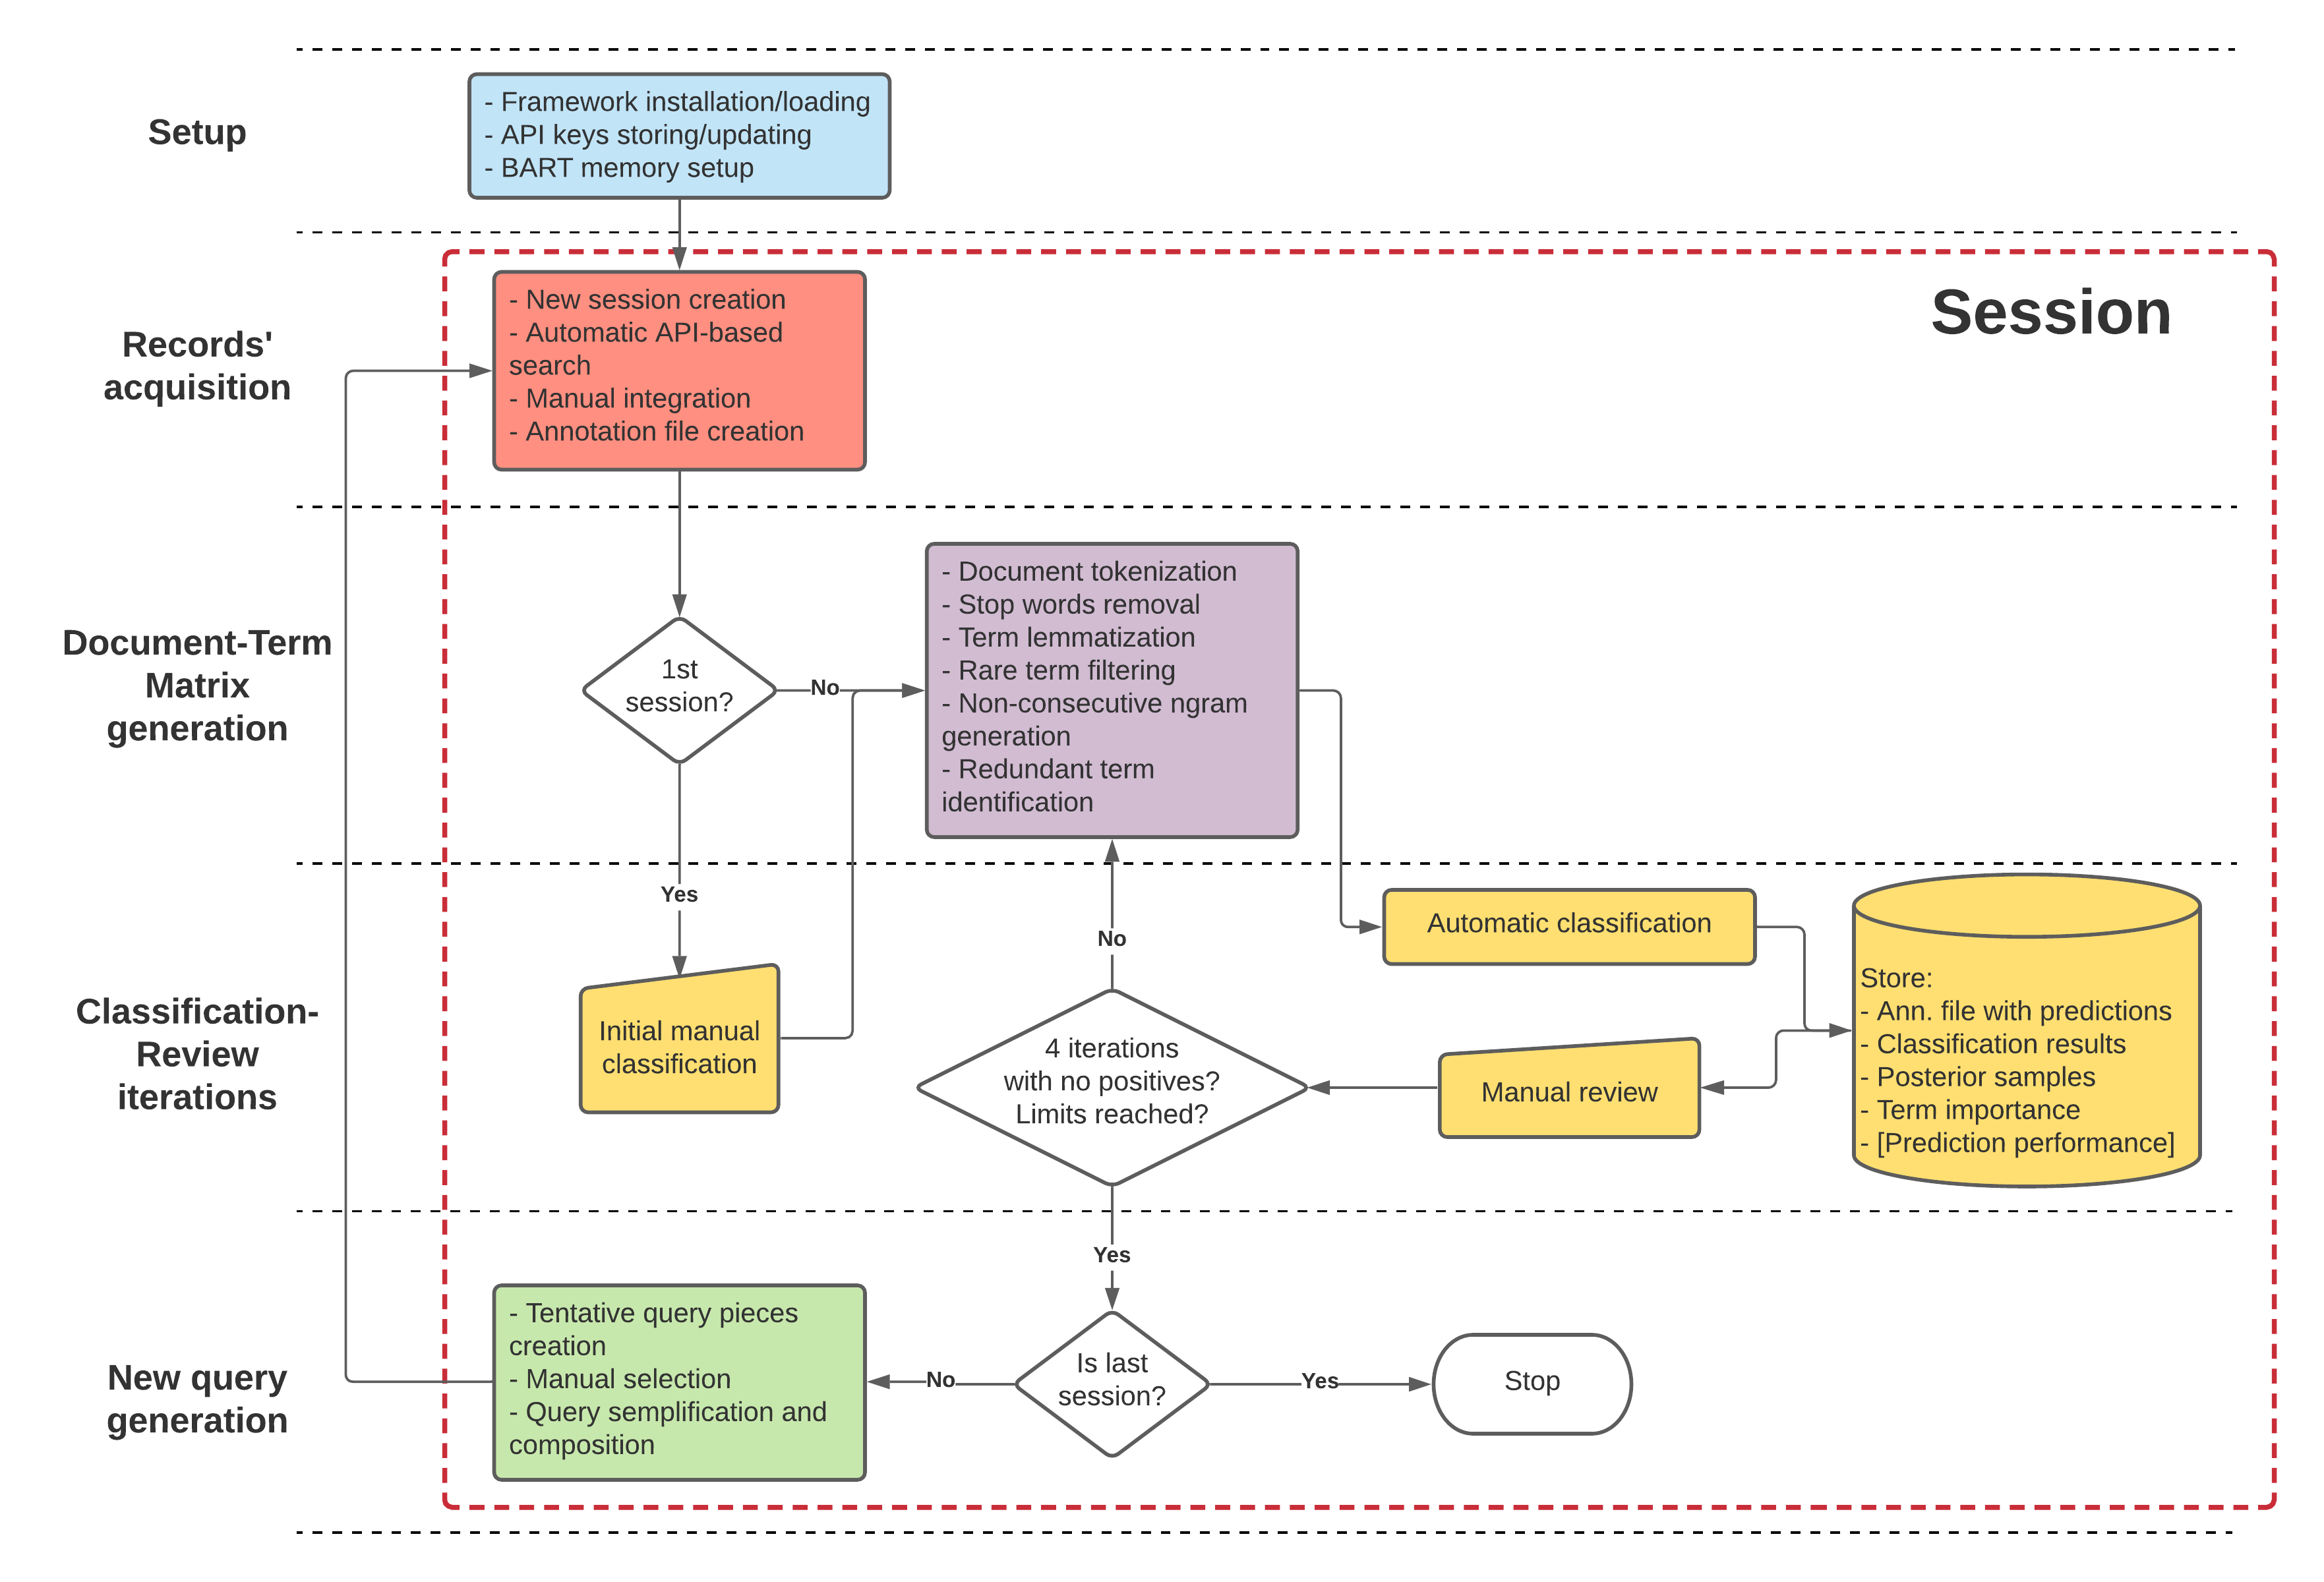
\includegraphics[width=1\linewidth]{methods_diagram} \caption{Figure 1.Framework's visual depiction.}\label{fig:method_diagram}
\end{figure}

\hypertarget{records-acquisition-and-initial-labelling}{%
\subsection{Record's acquisition and initial
labelling}\label{records-acquisition-and-initial-labelling}}

We built a set of tools to let users automatically search and download
citation data from three major scientific databases (``sources''):
Pubmed (\url{https://pubmed.ncbi.nlm.nih.gov/}), Web Of Science (WOS,
\url{https://apps.webofknowledge.com/}) and the Institute of Electrical
and Electronics Engineers (IEEE,
\url{https://ieeexplore.ieee.org/Xplore/home.jsp}). The framework takes
care of authorization management for non-open databases like WOS and
IEEE. It is also possible to download and import records in the
framework manually; this is particularly useful to acquire records from
the SCOPUS (\url{https://www.scopus.com/}) and EMBASE databases
(\url{https://www.embase.com/}), for which a comprehensive API interface
was not easy to build. An extra manual search was necessary also for
Pubmed, since the API and the web interface have different rule
expansion algorithms and return slightly different results ({`NCBI
Insights : Updated Pubmed e-Utilities Coming in April 2022!'}, n.d.). A
short guide on how to set up the framework for each supported database
is available in Supplemental Material S3.\\
The acquired records are merged into a single database, resolving
duplicates and different formatting between sources. The records are
ordered according to the frequency of the positive query terms (e.g.,
not preceded by a \(NOT\) modifier) in the title and abstract (``simple
query ordering'').\\
The researcher is then asked to label a number of records to create the
``initial training set'' needed to start the automatic classification.
We suggest manually labelling the first 250 records (see
``hyperparameter optimization'' later). The simple query ordering
increases the positivity rate in the initial training set (Wallace,
Small, et al. 2010), which provide higher sensitivity during automatic
classification (Chawla, Japkowicz, and Kotcz 2004).

\hypertarget{text-feature-extraction}{%
\subsection{Text feature extraction}\label{text-feature-extraction}}

The collected citation data have a number of fields characterising a
scientific publication. The framework models the relevance of a record
based on the following fields: title, abstract, authors, keywords, MESH
terms (Lipscomb 2000). A series of Natural Language Processing (NLP)
techniques (Baeza-Yates, Ribeiro-Neto, et al. 1999; Marshall and Wallace
2019; Ananiadou and McNaught 2006) are employed to transform the textual
information in these fields into features for machine learning through a
bag-of-words approach (Marshall and Wallace 2019). The processing of
free text fields (title, abstract) includes: tokenization (i.e.,
extracting the terms), common stopwords (i.e., sentence components
bringing no meaning) removal, part-of-speech filtering (only nouns,
adjectives, verbs and untagged terms are retained), and lemmatization of
the terms (i.e., reduction to their base grammar form). Text processing
for authors, keywords and MESH terms identifies logical units (e.g.,
author's full names, composite keywords) and extracts them.\\
Terms appearing in less than 5\% of the labelled documents are removed
from negative records. All terms in the positive set are kept to
increase sensitivity at the cost of specificity.\\
Some terms tend to co-appear in records (non-consecutive ngrams,
nc-ngrams), often carrying a particular meaning when copresent. To
detect nc-ngrams, we generated a word network representation (Francois
Rousseau 2015) posing edges between terms with a cosine similarity in
terms of record co-occurrence \textgreater{} 0.5. We extracted the
maximal cliques in the network (Eppstein, Löffler, and Strash 2010)
representing highly correlated groups of terms; These groups of terms
are added to the data set as individual features. Only nc-ngrams
comprising a maximum of ten terms are kept.\\
A second network is built using a co-occurrence threshold of 0.9. In
this case, the cliques represent terms that always appear together and
therefore can be considered redundant (i.e., they do not need to be
considered separately). These terms are merged to increase computation
efficiency and reduce overfitting.\\
The output is a Document-Term Matrix (DTM), with \(N_d\) rows
representing the records (\(D_i\)), \(N_t\) terms column for the
\(t_{field}\) terms (divided by record field) and \({0,1}\) values
whether \(t_{field} \in D_i\). We also enriched the DTM with features
referencing the number of terms in each field to help the model scale
term importance based on the field length.

\hypertarget{label-prediction}{%
\subsection{Label prediction}\label{label-prediction}}

We used a Bayesian Additive Regression Trees (BART) machine learning
``classification model'' (Chipman et al. 2010) (in the implementation of
Kapelner and Bleich 2013) to predict the probability of a record of
being relevant, given the information coded into the enriched DTM and
the initial training set. We set up the BART model to use 2000 MCMC
iterations (after 250 burn-in iterations) and 50 trees; we used a \(k\)
value of 2 to regularize extreme prediction and let the model use
missing fields in the DTM as features (Kapelner and Bleich 2015).
Positive records are oversampled ten times to increase sensitivity
(Batista, Prati, and Monard 2004).\\
The output is a posterior predictive distribution (PPD) for each record
describing its probability of being relevant (i.e., a positive match).
An ensemble of ten models was fitted to improve prediction stability by
averaging the PPD between models (Zhou 2021; Dietterich 2000).\\

To assign the labels, we employed an ``active learning'' Miwa et al.
(2014) approach, where a human reviews a specific subset of predictions
made from the machine, which is then retrained on the manually reviewed
data set. This process proceeds iteratively, decreasing prediction
uncertainty.\\
Label assignment is done through the identification of an ``uncertainty
zone'' whose construction is possible thanks to the Bayesian nature of
BART, which provides full PPDs instead of point-wise predictions for
each record.\\
To describe the process formally, we define

\[\pi_i = \frac{1}{M}\sum_{j=1}^M Pr(L_i = \text{1}|DTM,m_j)\]

as the PPD of a record \(D_i\) being relevant (i.e, having a positive
label, \(L_i = 1\)), averaging the PPDs of the ensemble of \(M=10\)
models \(m\), and

\[
\begin{aligned}
\pi_{i,l} = \{\pi_i : Pr(\pi_i) = 1\%\}\\
\pi_{i,u} = \{\pi_i : Pr(\pi_i) = 99\%\}
\end{aligned}
\]

as respectively the lower and upper boundaries of the 98\% quantile
interval of \(\pi_i\) (98\% Predictive Interval, 98\% PrI).\\
Then we identify the ``uncertainty zone'' as

\[U_\pi=[\max\vec{\pi}_{u}^-, \min\vec{\pi}_{l}^+]\] with
\(\vec{\pi}_{u}^-\) being the vector of \(\pi_{i,u}\) with a negative
label and \(\vec{\pi}_{l}^+\) the vector of \(\pi_{i,l}\) with a
positive label. That is, \(U_\pi\) defines a range of values between the
smallest \(\pi_{i,l}\) in the set of already labelled positive records
\(L_p\) and the largest \(pi_{i,u}\) related to the negative ones
\(L_n\), noting that the two limits can appear in any order.\\
Consequently, a record \(D_i\) will be labelled as positive if

\[\pi_{i,l} > \max_{\pi \in U_\pi} \pi\]

that is, the record lower 98\% PrI boundary should be higher than every
value in the uncertainty zone. In other words, for a record to be
labelled positive, its PPD should be within the range of the mixture of
PPD of the previously labelled positive records and not cross the
distributions of the negative records.\\
Conversely, a record is labelled as negative if

\[\pi_{i,u} < \min_{\pi \in U_\pi} \pi\]

All other records are labelled as ``uncertain''.

Manual review is then necessary for: 1) uncertain records, 2) positive
records (to avoid false positives), 3) records whose predicted label
differs from the existing manual one. The last case helps identify human
errors or inconsistent labelling criteria.

The automatic classification and the manual review steps alternate in a
loop (CR iterations) until no new positive matches are found in four
consecutive iterations.

\hypertarget{relevant-term-extraction}{%
\subsection{Relevant term extraction}\label{relevant-term-extraction}}

BART model it is possible to extract the proportion of times a term was
used in a posterior tree over the sum of total inclusions of all
variables (Kapelner and Bleich 2013), as a measure of feature importance
for the model. We extracted the terms, the part of the citation data
they were used in, the average ``inclusion rate'' among the ensemble
models (over 10,000 inclusions) and its ratio over the standard
deviation of this inclusion (inclusion stability, IS). For each term we
ran a Poisson regression to get its linear association with a positive
label and reported it as Relative Risk (RR) with the number of standard
errors as significance index (Statistic); the comparison between the
inclusion rate in the BART models and the linear association allows to
spot relevant non-linear effects (i.e, the feature is relevant only in
association with others). We reported in the Results only the first (in
order of inclusion rate) 15 terms with IS \textgreater{} 1.5 while the
first fifty terms regardless of inclusion stability are reported in
Supplemental Material S2.

\hypertarget{new-search-query-generation}{%
\subsection{New search query
generation}\label{new-search-query-generation}}

We created an algorithm that generates a new search query to acquire
further relevant publications missed during the first search, possibly
at a reasonable cost in specificity (i.e., a higher number of negative
results).\\
The algorithm encompasses a number of steps:

\begin{itemize}
\tightlist
\item
  We fit a partition tree (Therneau and Atkinson 2019) between the DTM
  and 800 samples from the PPD; if a term is present multiple times in
  the DTM (e.g., both title and abstract), they are counted just one,
  and field term count features are removed. This step generates a list
  of rules composed by \(AND\)/\(NOT\) ``conditions'' made of
  terms/authors/keywords/MESH tokens, which together identify a group of
  records.
\item
  For each rule, negative conditions (i.e., \(NOT\) statements) are
  added iteratively, starting from the most specific one, until no
  conditions are found that would not also remove positive records.
\item
  The extended set of rules is sorted by positive-negative record
  difference in descending order. The cumulative number of unique
  positive records is computed and used to group the rules. Rules inside
  each group are ordered by specificity.
\item
  The researcher is then asked to review the rule groups, selecting one
  or more rules (useful if they convey different meaning) from each, or
  edit them (in case too specific positive or negative conditions were
  included). It is possible to exclude a group of rules altogether,
  especially those with the worse sensitivity/specificity ratio.
\item
  The selected rules are joined together by \(OR\) statements, defining
  a subset of records with a sensibly higher proportion of positive
  records than the original one.
\item
  Redundant rules (i.e., rules whose positive records are already
  included in more specific ones) and conditions (i.e., conditions that
  once removed do not decrease the total number of positive or do not
  increase the negative records) are removed.
\item
  Finally, the rules are re-elaborated in a query usable on the major
  scientific databases.
\end{itemize}

Since the algorithm is data-driven, it creates queries that effectively
select positive records from the input data set but may be not specific
enough once applied to actual research databases. Therefore we appended
an extra subquery in \(AND\), which specifies the general topics of our
search and delimitates the search domain.\\
The new query was used to initiate a second search session.

\hypertarget{performance-evaluation}{%
\subsection{Performance evaluation}\label{performance-evaluation}}

We trained a simple Bayesian logistic regression (surrogate model) on
the reviewed records to evaluate the classification model consistency
(see Discussion for the theoretical justification). The surrogate model
uses as predictor the lower bound of the 98\% PrI of the records' PPD
with weakly regularizing, robust priors for the intercept (Student T
with \(\nu=3,\mu=0,\sigma=2.5\)) and the linear coefficient (Student T
with \(\nu=3,\mu=0,\sigma=1.5\)).\\
The quality of the model was evaluated through Bayesian \(R^2\) (Gelman
et al. 2019), of which we reported the posterior median and 90\%
Credible Interval {[}90\% CrI{]}. The \(R^2\) also provides an
evaluation of the consistency of the original classification model.
Given that this model is conditional only on the BART predictions and
not on the DTM, it is characterized by more uncertainty, providing
plausible worst-case scenarios.\\
The surrogate model is then used to generate the predictive cumulative
distribution of the number of total positive records in the whole data
set. This distribution allows estimating the expected total posterior
``Sensitivity'' and ``Efficiency'' of the classification model in the
full (unreviewed) data set. Efficiency is summarised by the ``Work saved
over random'' (WSoR) statistic: one minus the ratio between the number
of record manually reviewed and those that would be required to find the
same number of positives if classification was performed choosing
records randomly; this last quantity is estimated through a negative
hypergeometric distribution (Chae 1993) over the predicted amount of
positive records.\\
For the number of predicted positive records, the sensitivity and the
efficiency, we reported the ``truncated 90\% PrI'' {[}trunc. 90\%
PrI{]}, which is the uncertainty interval bounded at the number of
observed total positive records (i.e., there cannot be less predicted
positive records than observed).

\hypertarget{hyperparameter-evaluation}{%
\subsection{Hyperparameter evaluation}\label{hyperparameter-evaluation}}

Our classification algorithm has a number of hyperparameters:

\begin{itemize}
\tightlist
\item
  Size of the initial training set: 50, 100, 250, 500 records;
\item
  Number of models in the ensemble: 1, 5, 10, 20, 40, 60 repetitions;
\item
  Oversampling rate of positive records: (1x (i.e., no oversampling),
  10x, 20x;
\item
  PrI quantiles for building the uncertainty zone: 80\%, 90\%, 98\%;
\item
  Source of randomness between models in the ensemble: MCMC sampling
  only (Robert, Casella, and Casella 2004), MCMC plus data bootstrapping
  (Breiman 1996) of the training set.
\end{itemize}

To evaluate the hyperparameter effect of performance, we set up a ``grid
search'' (Claesen and De Moor 2015; L. Yang and Shami 2020) on a
prelabelled ``validation set'' made of the first 1200 records from the
first session data set. The framework tested each hyperparameter
combination until four CR iterations with no positive records were
returned or the whole data set got labelled.\\
For each combination, a performance score was computed as the product of
``Efficiency'' (1 minus the ratio of records that required review over
the total) and ``Sensitivity'' (number of positive records found over
the total of positives). We then identified homogeneous ``performance
clusters'' of scores given hyperparameter values using a partition tree
(Therneau and Atkinson 2019). For the rest of the study, we used the
best hyperparameter set in terms of Sensitivity followed by Efficiency
from the cluster with the highest average score.\\

\hypertarget{results}{%
\section{Results}\label{results}}

\hypertarget{first-session}{%
\subsection{First session}\label{first-session}}

The initial search query for the example topic was:\\

\emph{((model OR models OR modeling OR network OR networks) AND
(dissemination OR transmission OR spread OR diffusion) AND (nosocomial
OR hospital OR ``long-term-care'' OR ``long term care'' OR ``longterm
care'' OR ``long-term care'' OR ``healthcare associated'') AND
(infection OR resistance OR resistant))}

selecting only results between 2010 and 2020 (included). Results were
collected from Pubmed, WOS, IEEE, EMBASE and SCOPUS, using the framework
tools as described in Methods and Supplemental Material S1.

The first search session returned a total of 27600 records, specifically
12719 (71.6\% of the total) records from the EMBASE database, followed
by 9546 (53.8\%) from Pubmed, 3175 (17.9\%) from SCOPUS, 2100 (11.8\%)
from WOS, and 60 (0.34\%) from IEEE (Table 1). There were various
degrees of overlapping between sources, with the 38.4\% of records being
present in more than one database and EMBASE and IEEE being the
databases with the higher uniqueness ratios. The final data set was
composed by 17755 unique records.\\
The first 250 records (based on ``simple query ordering'') were manually
labeled. Of these 43 (17.2\%) were labeled as positive, and 207 (82.8\%)
as negative.

\begin{table}[!h]

\caption{\label{tab:Table 1}\textbf{Table 1}. Distribution of retrieved records by source and session. For each source it is reported the number of records, percentage over the session total (after removing duplicates), and number or records specific for a source as absolute value and as percentage over the source total. All session shows records after joining and deduplication of the Session 1 and Session 2 data set.}
\centering
\resizebox{\linewidth}{!}{
\begin{tabular}[t]{llrlrl}
\toprule
Session & Source & Records & \% over total & Source specific records & \% over source total\\
\midrule
\cellcolor{gray!6}{Session1} & \cellcolor{gray!6}{Total} & \cellcolor{gray!6}{17755} & \cellcolor{gray!6}{} & \cellcolor{gray!6}{} & \cellcolor{gray!6}{}\\
 & Embase & 12719 & 71.6\% & 6683 & 52.5\%\\
\cellcolor{gray!6}{} & \cellcolor{gray!6}{Pubmed} & \cellcolor{gray!6}{9546} & \cellcolor{gray!6}{53.8\%} & \cellcolor{gray!6}{3457} & \cellcolor{gray!6}{36.2\%}\\
 & Scopus & 3175 & 17.9\% & 298 & 9.39\%\\
\cellcolor{gray!6}{} & \cellcolor{gray!6}{WOS} & \cellcolor{gray!6}{2100} & \cellcolor{gray!6}{11.8\%} & \cellcolor{gray!6}{473} & \cellcolor{gray!6}{22.5\%}\\
\addlinespace
 & IEEE & 60 & 0.34\% & 29 & 48.3\%\\
\cellcolor{gray!6}{Session2} & \cellcolor{gray!6}{Total} & \cellcolor{gray!6}{82579} & \cellcolor{gray!6}{} & \cellcolor{gray!6}{} & \cellcolor{gray!6}{}\\
 & Embase & 48396 & 58.6\% & 40826 & 84.4\%\\
\cellcolor{gray!6}{} & \cellcolor{gray!6}{Pubmed} & \cellcolor{gray!6}{28811} & \cellcolor{gray!6}{34.9\%} & \cellcolor{gray!6}{18021} & \cellcolor{gray!6}{62.5\%}\\
 & Scopus & 17070 & 20.7\% & 4908 & 28.8\%\\
\addlinespace
\cellcolor{gray!6}{} & \cellcolor{gray!6}{WOS} & \cellcolor{gray!6}{12956} & \cellcolor{gray!6}{15.7\%} & \cellcolor{gray!6}{2817} & \cellcolor{gray!6}{21.7\%}\\
 & IEEE & 61 & 0.074\% & 22 & 36.1\%\\
\cellcolor{gray!6}{All Sessions} & \cellcolor{gray!6}{Total} & \cellcolor{gray!6}{98371} & \cellcolor{gray!6}{} & \cellcolor{gray!6}{} & \cellcolor{gray!6}{}\\
 & Embase & 59604 & 60.6\% & 46942 & 78.8\%\\
\cellcolor{gray!6}{} & \cellcolor{gray!6}{Pubmed} & \cellcolor{gray!6}{37278} & \cellcolor{gray!6}{37.9\%} & \cellcolor{gray!6}{21371} & \cellcolor{gray!6}{57.3\%}\\
\addlinespace
 & Scopus & 19353 & 19.7\% & 5181 & 26.8\%\\
\cellcolor{gray!6}{} & \cellcolor{gray!6}{WOS} & \cellcolor{gray!6}{14367} & \cellcolor{gray!6}{14.6\%} & \cellcolor{gray!6}{3175} & \cellcolor{gray!6}{22.1\%}\\
 & IEEE & 108 & 0.11\% & 48 & 44.4\%\\
\bottomrule
\end{tabular}}
\end{table}

The labeled records were used to train the Bayesian classification model
used to label the remaining records. After seven classification and
review (CR) iterations (three resulting in new positive matches and four
extra replications to account for stochastic variability), a total of
101 positives matches were found, requiring manual review of 766 records
(13.2\% positivity rate).\\
It is possible to observe how the number of records that required manual
review dropped rapidly between iterations (Table 2), indicating that the
engine was converging while the uncertainties were resolved.\\
This phenomenon is better depicted in Fig. 1 of the Supplemental
Material S2, showing the mixture distribution of the PPDs of the
records, specifically for the reviewed positive and negative records,
and for records that need manual review after the classification step:
it can be noticed how the distribution of the uncertain records shrinked
(ie., gets concentrated in a shorter probability range) and shifted
toward the negative zone as more positive matches are found and
reviewed.

\begin{table}[!h]

\caption{\label{tab:Table 2}\textbf{Table 2}. Results of the automatic classification and manual review rounds. For each iteration, the cumulative number of positives and negative records and their sum (Total labelled) and percentage over total are shown. Also, the number of changes after review and their description is reported."Unlab." indicates unlabelled records marked for review. For each Iteration, also the number of features used by the engine is reported. The first row reports the results of the initial manual labelling of records, which acted as input for the automatic classification in Iteration 1. In Session 2, the engine uses the labels at the end of Session 1 to classify the newly added records.}
\centering
\resizebox{\linewidth}{!}{
\begin{tabular}[t]{llrrlrrrrrr}
\toprule
Session & Iteration & Positives & Negatives & Total labelled (\%) & Unlab. -> y & Unlab. -> n & Unlab. -> * & n -> y & Changes & N. features\\
\midrule
\cellcolor{gray!6}{Session1 (n = 17755)} & \cellcolor{gray!6}{Initial labelling} & \cellcolor{gray!6}{43} & \cellcolor{gray!6}{207} & \cellcolor{gray!6}{250 (1.41\%)} & \cellcolor{gray!6}{43} & \cellcolor{gray!6}{207} & \cellcolor{gray!6}{0} & \cellcolor{gray!6}{0} & \cellcolor{gray!6}{250} & \cellcolor{gray!6}{2289}\\
 & 1 & 93 & 529 & 622 (3.5\%) & 50 & 322 & 0 & 0 & 372 & 2289\\
\cellcolor{gray!6}{} & \cellcolor{gray!6}{2} & \cellcolor{gray!6}{100} & \cellcolor{gray!6}{614} & \cellcolor{gray!6}{714 (4.02\%)} & \cellcolor{gray!6}{6} & \cellcolor{gray!6}{86} & \cellcolor{gray!6}{0} & \cellcolor{gray!6}{1} & \cellcolor{gray!6}{93} & \cellcolor{gray!6}{3750}\\
 & 3 & 101 & 625 & 726 (4.09\%) & 1 & 11 & 0 & 0 & 12 & 3834\\
\cellcolor{gray!6}{} & \cellcolor{gray!6}{4} & \cellcolor{gray!6}{101} & \cellcolor{gray!6}{648} & \cellcolor{gray!6}{749 (4.22\%)} & \cellcolor{gray!6}{0} & \cellcolor{gray!6}{23} & \cellcolor{gray!6}{0} & \cellcolor{gray!6}{0} & \cellcolor{gray!6}{23} & \cellcolor{gray!6}{3856}\\
\addlinespace
 & 5 & 101 & 651 & 752 (4.24\%) & 0 & 3 & 0 & 0 & 3 & 3856\\
\cellcolor{gray!6}{} & \cellcolor{gray!6}{6} & \cellcolor{gray!6}{101} & \cellcolor{gray!6}{660} & \cellcolor{gray!6}{761 (4.29\%)} & \cellcolor{gray!6}{0} & \cellcolor{gray!6}{9} & \cellcolor{gray!6}{0} & \cellcolor{gray!6}{0} & \cellcolor{gray!6}{9} & \cellcolor{gray!6}{3856}\\
 & 7 & 101 & 665 & 766 (4.31\%) & 0 & 5 & 0 & 0 & 5 & 3856\\
\cellcolor{gray!6}{Session2 (n = 98371)} & \cellcolor{gray!6}{1} & \cellcolor{gray!6}{106} & \cellcolor{gray!6}{934} & \cellcolor{gray!6}{1040 (1.06\%)} & \cellcolor{gray!6}{5} & \cellcolor{gray!6}{270} & \cellcolor{gray!6}{998} & \cellcolor{gray!6}{0} & \cellcolor{gray!6}{1273} & \cellcolor{gray!6}{4729}\\
 & 2 & 107 & 1123 & 1230 (1.25\%) & 1 & 189 & 0 & 0 & 190 & 4729\\
\addlinespace
\cellcolor{gray!6}{} & \cellcolor{gray!6}{3} & \cellcolor{gray!6}{107} & \cellcolor{gray!6}{1176} & \cellcolor{gray!6}{1283 (1.3\%)} & \cellcolor{gray!6}{0} & \cellcolor{gray!6}{53} & \cellcolor{gray!6}{0} & \cellcolor{gray!6}{0} & \cellcolor{gray!6}{53} & \cellcolor{gray!6}{4733}\\
 & 4 & 107 & 1200 & 1307 (1.33\%) & 0 & 24 & 0 & 0 & 24 & 4729\\
\cellcolor{gray!6}{} & \cellcolor{gray!6}{5} & \cellcolor{gray!6}{107} & \cellcolor{gray!6}{1209} & \cellcolor{gray!6}{1316 (1.34\%)} & \cellcolor{gray!6}{0} & \cellcolor{gray!6}{9} & \cellcolor{gray!6}{0} & \cellcolor{gray!6}{0} & \cellcolor{gray!6}{9} & \cellcolor{gray!6}{4729}\\
 & 6 & 107 & 1226 & 1333 (1.36\%) & 0 & 17 & 0 & 0 & 17 & 4729\\
\bottomrule
\end{tabular}}
\end{table}

We extracted the 15 term more relevant for the classification model,
described as: Term (citation part): Inclusion Rate (Inclusion Stability)
{[}linear Relative Risk, Statistic{]}.

Patient Transport (Keyword): 61.2 (3.77) {[}99.1, 21.3{]}, Transfer
(Abstract): 57 (3.93) {[}22.5, 15.4{]}, Network (Title): 56.5 (2.91)
{[}18, 14.2{]}, Network \& Patient (Abstract): 54.2 (4.66) {[}26.3,
15.2{]}, Donker T (Author): 53.5 (4.56) {[}159, 16.5{]}, Worker
(Abstract): 50 (3.33) {[}0.421, -1.21{]}, Hospitals (Keyword): 49.8
(4.31) {[}27.8, 16.5{]}, Movement (Abstract): 47.8 (2.7) {[}27.2, 15{]},
Spread (Title): 46.6 (2.25) {[}16.2, 12.1{]}, Facility (Abstract): 45
(2.22) {[}19.6, 14.8{]}, Orange County (Keyword): 44.3 (3.19) {[}199,
17.2{]}, Conduct (Abstract): 42.6 (3.7) {[}0.221, -2.57{]}, Patient
(Abstract): 42 (3.61) {[}27.6, 7.23{]}, Perform (Abstract): 41.9 (2.38)
{[}0.342, -2.55{]}, Hospital (Title): 39 (1.95) {[}12.5, 12.5{]}.

The ``\&'' indicates nc-ngrams, i.e., terms strongly co-occurrent in the
documents.\\
The engine was able to pick up the central concept of the research
topic, i.e., ``patient transport'' or ``transfer'' through a ``network''
of ``facility''ies that facilitates the ``spread'' of infections, and
even one of the authors of this study (Donker T.) as well as the region
of interest (``Orange County'') of another research group active on the
topic of pathogen spreading over hospital networks. Some terms were
considered highly relevant by the BART models (e.g., ``Worker'' in 6th
position out of more than 3800 terms considered) although in a simpler
linear model their effect would be hardly significant (statistic: -1.21
s.e.); these are terms which are relevant only in conjunction with other
terms but not by themselves, highlighting the extra predictive power
brought by using advanced, non-linear machine learning.\\
A more extensive set of terms is presented in Table 1 of Supplemental
Material S2.

\hypertarget{second-session}{%
\subsection{Second session}\label{second-session}}

The results of the first classification session were used to create a
second, data-driven query with the purpose of performing a more
large-spectrum search to find records which may have escape the first
search session. The resulting query was the following:\\

\emph{(((Donker T) NOT (bacterium isolate)) OR ((network patient) AND
(resistant staphylococcus aureus) NOT (monte carlo) NOT isolation) OR
(facility AND (network patient) AND regional NOT hospitals NOT increase
NOT (patient transport) NOT (control infection use)) OR ((patient
transport) NOT (Donker T) NOT worker) OR (hospitals AND (network
patient) NOT (patient transport) NOT regional NOT clinical) OR (facility
AND (network patient) NOT hospitals NOT (patient transport) NOT regional
NOT prevention NOT medical) OR ((healthcare facility) NOT (Donker T) NOT
worker NOT positive) OR (hospitals NOT (network patient) NOT medical NOT
environmental NOT outcome NOT global) OR ((network patient) NOT facility
NOT hospitals NOT (patient transport) NOT therapy NOT global)) AND
((antimicrobial resistance) OR (healthcare infection))}

The final piece \emph{AND ((antimicrobial resistance) OR (healthcare
infection)} was added manually to better define the search domain, since
the algorithm was trained on documents that were all more or less
related to these topics.\\
The generated query also provides a more nuanced understanding of the
engine's internal classification logic, and this is helpful to spot
possible biases in the model.\\

The search was done with the same year filter and procedures of the
first session.\\

The new search produced 107294 records (Table 1), of which 48396
(58.6\%) from the EMBASE, followed by 28811 (34.9\%) from Pubmed, 17070
(20.7\%) from SCOPUS, 12956 (15.7\%) from WOS, and 61 (0.074\%) from
IEEE; compared with the first session, the relative weight of EMBASE and
Pubmed was decreased, while the amount of content specificity was
greatly increased, as it was for SCOPUS. After removal of duplicates,
82579 unique records were obtained. Once joined with the session 1
records and removal of duplicates, we obtained 98371 unique records,
with just 1963 shared records between searches, that is the 2\%. The
percentage of records shared by two or more source dropped to 22\%.

Six CR rounds were necessary to complete the second session
classification, with just 6 new positive found after reviewing 568 extra
records. The first CR iteration required the user to review a
substantial number of records (1,273), but just labelling 275 of them
(the canonical 250 plus 25 that were already labelled during the
framework hyperparameter tuning) was sufficient to drop this number to
just 190 in the subsequent round. An evaluation of the convergence
(Figure 1, Supplemental Material S2) showed that, in addition to the
dynamics already observed in session 1 (shrinkage and negative shift), a
second mode appeared in the mixture distribution of the records to be
reviewed, centred in a highly positive zone. The interpretation is that
as the number of negative training records increases, the engine gets
more and more skeptical and asks to review even some records labelled as
positive in the initial training set generated during Session 1. This
behaviour can be useful to spot classification errors and
inconsistencies. Considering both sessions, 1333 records were manually
reviewed and 107 (8.03\%) confirmed positive matches were found.

Again, the evaluation of the inclusion rate of the terms showed that the
engine was quite capable of internalizing the concepts behind the
research topic A subsample of the relevant terms used by the model in
the second session is reported in Table 2 of Supplemental Material S2.

\hypertarget{hyperparameter-selection}{%
\subsection{Hyperparameter selection}\label{hyperparameter-selection}}

As described in the methods, the selection of hyperparameters was
achieved via evaluation of sensibility and efficiency through a grid
search on a validation set of 1200 manually labelled records. The
analysis suggested the following combination of parameters as the best
performing: an initial input of 250 labelled records with 10x positive
matches oversampling, an averaged ensemble of 10 models, no
bootstrapping and an uncertainty zone defined by the 98\% predictive
interval. This combination of parameters was associated with a
sensitivity of 98.8\% (81 / 82 positive matches found) and efficiency of
61.5\% (462 / 1200 records evaluated). The detailed results of the
hyperparameter tuning ananlysis are reported in Table 3 of Supplemental
Material S2. Figure 2 in Supplemental Material S2 demonstrates that the
positive record oversampling rate, the number of ensemble models and the
size of the initial training set were the parameters that mostly
impacted performance.

\hypertarget{performance-evaluation-1}{%
\subsection{Performance evaluation}\label{performance-evaluation-1}}

To evaluate the theoretical performance of the engine, a surrogate
Bayesian logistic regression model was trained on the manually reviewed
labels using only the lower bound of the record PPDs as predictor (see
Methods for the details). The surrogate model showed the high predictive
power of the scores produced by the classification model (Bayesian R2:
98.1\% {[}97.4\%, 98.3\%{]} for session 1 and 98.2\% {[}97.6\%,
98.3\%{]} for session 2).\\

Figure 2 presents the actual and predicted (from the surrogate model)
cumulative number of positive matches, ordered by the initial simple
ordering query: the median of surrogate models' cumulative predictive
distributions matches quite well the actual number of positive records
found. It is striking how many more records would have needed to be
evaluated manually to find the same number of positive matches without
using a smart classification tool, with some positive matches found
close to the end of the heuristically ordered list of records.\\

Table 3 shows various performance indexes for both sessions, both
descriptive (Total records, Reviewed records, Observed positive matches)
and estimated through the surrogate model (Expected efficiency,
Predicted positive matches, Expected sensitivity, \(R^2\)).\\
In session 1 we observe an expected total number of positives of 101
{[}101, 108{]} for an estimated sensitivity of 100\% {[}93.5\%, 100\%{]}
and efficiency of 95.6\% {[}95.3\%, 95.7\%{]}. In session 2 we observed
a drop in the expected sensitivity, especially in the lower credibility
boundary (97.3\% {[}72.8\%, 100\%{]}), due to the fact that as the
number of records grows, even a small probability of being a positive
match can translate, in the worst case scenario, into a relevant number
of missed positive matches (147 in this case). To ascertain that no
evident positives were missed, we evaluated 100 more records between the
unreviewed ones with the highest median predicted probability produced
by the engine and found no additional positive matches.\\

\begin{table}[!h]

\caption{\label{tab:Table 3}\textbf{Table 3}. Estimated performance summary. The table reports for each session, the number of reviewed records and the percentage over the total. Also, the posterior expected number of positive records, "Sensitivity" and "Efficiency" (as WSoR) are reported, with their 90\% PrI truncated to the observed realization in the dataset [trunc. PrI] (see. methods). Finally the median Bayesian $R^2$ [90\% CrI] of the logistic models is reported. PrI: Predictive Intervals; CrI: Credibility Intervals.}
\centering
\begin{tabular}[t]{lll}
\toprule
Indicator & Session 1 & Session 2\\
\midrule
\cellcolor{gray!6}{Total records} & \cellcolor{gray!6}{17755} & \cellcolor{gray!6}{98371}\\
Reviewed records (\% over total records) & 766 (4.31\%) & 1333 (1.36\%)\\
\cellcolor{gray!6}{Expected efficiency (over random) [trunc. 90\% PrI]} & \cellcolor{gray!6}{95.6\% [95.3\%, 95.7\%]} & \cellcolor{gray!6}{98.6\% [98.1\%, 98.6\%]}\\
Observed positive matches (\% over total records) & 101 (0.57\%) & 107 (0.11\%)\\
\cellcolor{gray!6}{Predicted positive matches [trunc. 90\% PrI]} & \cellcolor{gray!6}{101 [101, 108]} & \cellcolor{gray!6}{110 [107, 147]}\\
\addlinespace
Expected sensitivity [trunc. 90\% PrI] & 100\% [93.5\%, 100\%] & 97.3\% [72.8\%, 100\%]\\
\cellcolor{gray!6}{Simple Model $R^2$ [90\% CrI]} & \cellcolor{gray!6}{98.1\% [97.4\%, 98.3\%]} & \cellcolor{gray!6}{98.2\% [97.6\%, 98.3\%]}\\
\bottomrule
\end{tabular}
\end{table}

\begin{figure}
\centering
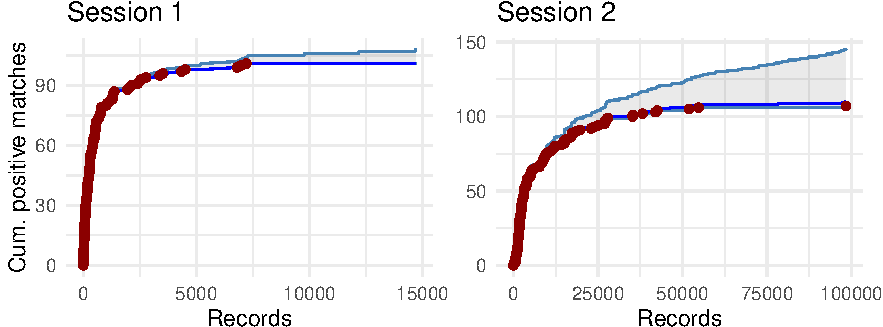
\includegraphics{Manuscript_files/figure-latex/performance plot-1.pdf}
\caption{\textbf{Figure 2}. Observed cumulative number of positive
matches (red dots) sorted by simple query ordering. The {[}trunc. 90\%
PrI{]} of the cumulative positive matches estimated by the logistic
Bayesian model is shown as shaded area delimited by the 95\% quantile of
the PrI and by the observed number of positive matches (light blue
lines). The median of the PrI is represented by a darker blue line.}
\end{figure}

\hypertarget{discussion}{%
\section{Discussion}\label{discussion}}

We propose a new integrated framework to help researchers collect and
screen scientific publications characterised by high performance and
versatility, joining the growing field of systematic review automation
(SRA) and helpers (SRH) tools (A. M. Cohen et al. 2006, 2010; Ananiadou
et al. 2009; O'Mara-Eves et al. 2015). This framework implements
standard approaches and uses ad-hoc solutions to deal with common SRA
issues. By freely sharing the tool as an open-source R package and by
following a modular design, we tried to adopt some of the so-called
Vienna Principles advocated by the International Collaboration for the
Automation of Systematic Reviews (ICASR) (E. Beller et al. 2018).\\
The framework consists of four main components: 1) an integrated
query-based citation search and management engine, 2) a Bayesian active
machine learning-based citation classifier, and 3) a data-driven search
query generation algorithm.\\

The framework's search engine module is capable of automatically
collecting citation data from three well-known scientific databases
(i.e., Pubmed, Web of Science, and the database of the Institute of
Electrical and Electronics Engineers) as well as process manually
downloaded results from both the two more (SCOPUS, EMBASE) databases. In
comparison, most SRH tools, commercial or free to use, rely either on
internal databases (e.g., Mendeley \url{https://www.mendeley.com/})
sometimes focusing just on a particular topic (Visser 2010) or on a
single external data source (Thomas and Brunton 2007; Poulter et al.
2008; Soto, Przybyła, and Ananiadou 2019).\\
Mixing different databases is fundamental to have a more comprehensive
view of the literature (Bajpai et al. 2011; Wilkins, Gillies, and Davies
2005; Woods and Trewheellar 1998): in our results, 18.7\% of the
positive matches found only in one of the different data sources, and no
positive record was present in all of them (data not shown).\\
The online search algorithms are efficient enough to manage tens of
thousands of search results, using various expedients to overcome the
limitations of online citation databases in terms of traffic and
download quotas. The results are then automatically organized,
deduplicated and arranged by ``simple query ordering'' in a uniform
corpus. The preliminary ordering allows to increase the positivity rate
in the initial training set (Wallace, Small, et al. 2010).\\

For the framework's record classification module, we employed an active
machine learning approach Miwa et al. (2014) based on the best practices
from other SRA studies but also bringing further improvements at various
levels.\\
The feature extractor module uses modern NLP techniques (Ananiadou and
McNaught 2006; K. B. Cohen and Hunter 2008) to transform text into input
data for machine learning. We did not include classical n-grams
(Schonlau and Guenther 2017), but we used network analysis to find
non-consecutive frequently associated terms, a generalisation of n-grams
relaxing the term adjacency assumption. This approach allows also to
find term connections across fields, for example a term having a
different relevancy if associated with a specific author. The same
technique but with different parameters was applied to merge redundant
terms to make model estimation more efficient and reduce noise.\\
The use of concurrency network-driven modelling of text is not new
(Francois Rousseau 2015; Violos et al. 2016; François Rousseau, Kiagias,
and Vazirgiannis 2015; Ohsawa, Benson, and Yachida 1998) and is a
valuable tool to extract semantic information not evident in one-word or
consecutive n-gram models.\\

The automatic classification algorithm is based on Bayesian Additive
Regression Trees (BART) (Chipman et al. 2010; Kapelner and Bleich 2013).
As with other boosted trees algorithms (Hastie, Tibshirani, and Friedman
2009), BART can explore complex non-linearities, perform variable
selection, manage missing data while sporting high performance in
predictive power.\\
However, its Bayesian foundation provides further benefits: less
sensitivity on hyperparameter choices, natural regularisation through
priors, and, especially, predictive distributions as output in place of
point-wise predictions (Soria-Olivas et al. 2011; Joo, Chung, and Seo
2020; Jospin et al. 2020). By selecting relatively tight prior
distributions, we discouraged excessively deep trees, long sequences of
trees, or extreme predicted probabilities, to decrease the risk of
overfitting.\\
The algorithm runs multiple replications of the model and averages their
predictive distributions creating an ``ensemble''; this technique has
been shown to improve out-of-sample predictive performance (Zhou 2021;
Dietterich 2000), as we were able to confirm during the hyperparameter
evaluation (Supplemental Material S2). Ensembling reduces the
uncertainty in the predictive distribution tails related to the
randomness in the MCMC fit (Robert, Casella, and Casella 2004),
generating a shift of probability mass towards the distribution centre
and stabilising it (i.e., decreasing variance without impacting bias).
On the other hand, just imposing robust uninformative priors against
extreme predictions would have decreased variance but also shifted the
distribution towards a non-decision zone, increasing bias (Hansen et al.
2000).\\
Since the number of model replications significantly impacts computation
times, we decided to use ten replicas, the lower value after which
performance stabilised during the hyperparameter evaluation.\\
We also investigated whether bootstrapping between replications (Breiman
1996) would improve performance, but, contrary to theory (Díez-Pastor et
al. 2015), it appeared to be slightly detrimental in our case
(Supplemental Material S2) compared to simple ensembling.\\

A low rate of relevant matches (class imbalance) is typical in
literature reviews (Sampson, Tetzlaff, and Urquhart 2011; Wallace,
Trikalinos, et al. 2010; O'Mara-Eves et al. 2015), and such strong
imbalance between positive and negative records can affect sensitivity
(Khoshgoftaar, Van Hulse, and Napolitano 2010; Chawla, Japkowicz, and
Kotcz 2004).\\
To overcome the problem, we oversampled (Batista, Prati, and Monard
2004) the positive records ten times before model fitting. Our
hyperparameter analysis showed that together with model ensembling, the
oversampling rate was the parameter with the highest impact on
performance.\\
A known risk with positive oversampling is the misclassification of
negative records (Ramezankhani et al. 2016). However, since all
predicted positives get manually reviewed in our approach, we are always
ensured to achieve 100\% specificity/positive predictive value: the only
price for the increased sensitivity due to oversampling is a larger
number of records to review.\\
An alternative to oversampling would be applying different weights
and/or cost to the classes (Abd Elrahman and Abraham 2013; Díez-Pastor
et al. 2015), but the BART implementation we used did not have this
feature; also, using simple oversampling permits broader compatibility
with different modelling engines (Galar et al. 2011; Roshan and Asadi
2020).\\
Finally, ordering the records by query term frequency (simple query
ordering) generates a far higher rate of relevant records in the initial
training set (17.2\%) compared to the overall data (0.11\%), and this
boosts the sensitivity of the model.\\

One of the central innovations we introduced is the concept of
``uncertainty zone'', whose implementation is possible thanks to the
Bayesian foundation of the classification model. This construct guides
the selection of the records to review, dynamically updating and
shrinking after every CR iteration, as more uncertain predictions are
evaluated (Supplemental Material S2 Fig. 1).\\
This approach overcomes the usual requirement of dataset-specific hard
thresholds in active machine learning, and also allows to review
multiple items at once between iterations (Laws and Schütze 2008; Miwa
et al. 2014; Zhu et al. 2010). The parameters our algorithm needs are
instead general and non task-specific, like the PPD intervals based on
which the uncertainty zone is built, and the maximum number of
iterations with no positive matches after which a session is concluded;
the hyperparameter evaluation shows that the algorithm is robust against
variations in these parameters and we expect the default values to
perform well on most datasets.\\
Since researchers are asked to review both records with a positive
predicted label and those inside the uncertainty zone, this method can
be considered as a unifying synthesis of the ``certainty'' and
``uncertainty'' paradigms of active learning (Miwa et al. 2014).\\

We evaluated performance as the capability of the screening procedure
(automatic classification plus manual review) to find the largest number
of relevant records while reviewing as few of them as possible (i.e.,
sensitivity \(\times\) efficiency).\\
We avoided the classic out-of-sample approaches like train-test
sampling, out-of-bag bootstrapping or cross-validation (Kohavi et al.
1995; James et al. 2013). Such methods primarily assume that the rate of
positivity is equal on average in every random subset of the data
(Tashman 2000); this uniformity is broken by how the initial training
set and the subsequent reviewed records are selected by the query-based
ordering and the active learning algorithm, determining a lower
positivity rate in the unlabelled records (Fig. 2). Also, a literature
corpus is unique per search query/database combination, and therefore
any out-of-sample performance estimate is not replicable since no new
data can be acquired related to the current corpus.\\
Instead, to estimate overall sensitivity, we employed simple Bayesian
regression (surrogate model) on the manually reviewed data to abstract
the classification model predictions and achieve a maximum entropy
(Harremoës and Topsøe 2001) estimate of the number of missed positive
matches among the unreviewed records in the whole dataset. This simple
surrogate model fitted the data very well (\(R^2\) consistently above
97\%) using just the lower 98\% PrI bound of the PPDs as predictor,
indicating predictive consistency in the classification model. The
surrogate model posterior predictive distribution could be exploited to
explore worse case scenarios in terms of sensitivity.\\

Our framework achieved very high sensitivity by screening a markedly
small fraction of all records, bringing a sensible reduction in
workload.\\
Based on the surrogate model, we predicted a predicted median
sensitivity of 100\% {[}93.5\%, 100\%{]} in the first session (screening
4.29\% of records) and of 97.3\% {[}73.8\%, 100\%{]} in the second
(screening 1.34\% of records): efficiency increased significantly in the
second session since only a few new positive matches were found, but
given the large number of records, uncertainty regarding sensitivity
also expectedly increased.\\
Both results are above the usual performance in the field (O'Mara-Eves
et al. 2015) and in line with the 92\% average sensitivity estimated
after human-only screening (Edwards et al. 2002). In one interesting
case, the model spotted a human-made misclassification error,
demonstrating its robustness and value as a second screener, a role
already suggested for SRA tools by previous studies (Frunza, Inkpen, and
Matwin 2010; Bekhuis and Demner-Fushman 2012, 2010). Finally, albeit the
simple query ordering already concentrated most of the relevant matches
in the first 20-25 thousand records, without the tool support some
relevant records would have required almost the complete data set to be
manually checked to be found.\\

The model took \textasciitilde5-20 minutes per iteration to perform
predictions in session 1 (17,755 documents) and 20-40 minutes in session
2 (98,371 documents) on an eight-core, 2.5 GHz, 16 GB RAM laptop from
2014; including manual record review, one session required 1-3 days of
work, for a total of 1-2 weeks for the whole process (including record
collection). That is a considerable saving of time compared to the
multiple months usually required for the screening phase of systematic
reviews (Bannach-Brown et al. 2019; Borah et al. 2017; Allen and Olkin
1999). To our knowledge, the amount of data processed
(\textasciitilde100.000 records) were larger than what is typical in
most SRA studies (O'Mara-Eves et al. 2015; Olorisade et al. 2016),
emphasising the reliability of the tool in real-world scenarios.\\

The last module of our framework is a data-driven query generation
algorithm. Creating an efficient and efficacious search query is a
complex task (Lefebvre et al. 2011; Hammerstrøm et al. 2010); it
requires building a combination of positive and negative terms to
maximise the number of relevant search results while minimising the
total number of records to review. Our solution joins a
sensitivity-driven subquery proposal engine based on concurrent decision
trees (Blanco-Justicia and Domingo-Ferrer 2019; Moore et al. 2018) built
on the BART ensemble PPD, with a human review step and an
efficiency-driven query builder. The aim is to generate a second query
that helps find records missed during the first session search. The
generated query allowed indeed to retrieve few more positive matches not
found in session 1, but at the cost of a significant increase in the
number of documents.\\
One interesting aspect of this functionality is that it provides a
human-readable overview of the classification rules learned by the
classification model, showing which combination of terms was
particularly relevant and even spotting authors and geographical
locations associated with the study topic. The generated query,
therefore, acted as a tool for machine learning explainability (Bhatt et
al. 2020; Burkart and Huber 2021), a feature useful to understand and
spot bias in black-box classification algorithms (Malhi, Knapic, and
Främling 2020); explainability is often required or even legally
mandatory for high-stake machine learning applications (Bibal et al.
2021, 2020).\\
It is important to note that this process is entirely data-driven. The
algorithm is only aware of the ``world'' defined by the data set used as
input, which is generated by a specific search query focused on a
particular topic. Therefore, the new query may not be specific enough
once applied to an unbounded search domain, returning an unmanageable
amount of unrelated results. The solution we found was to add another
component to the query, specifying the general topic (antimicrobial
resistance and healthcare-associated infections) of our research.\\

As reported, our framework builds on modularity. We designed it to
easily implement complete independence of the main modules in future
iterations, making it possible for users to add custom features like
citation search and parsing for other scientific databases, alternative
text processing algorithms or machine learning modules. We deem such
interoperability extremely relevant because the main strength of our
tool is the composition of many solutions and the general idea of
Bayesian active machine learning and the exploit of the derived
uncertainty in predictions. However, each of its components could
benefit considerably from the recent improvements in text mining.\\
For example, our text processing approach is quite simple, based on the
boolean bag-of-words paradigm, and indeed could be improved by more
nuanced text representations. It could be evaluated if feature
transformations like TF-IDF (Baeza-Yates, Ribeiro-Neto, et al. 1999;
Ananiadou and McNaught 2006) would be advantageous, even if we
hypothesise that tree-based classification algorithms like BART are
robust enough not to need such operations. Word embedding could be
instead worth exploring: this technique transforms terms in semantic
vectors derived from the surrounding text Minaee et al. (2021) and could
be used to eliminate semantically redundant terms or differentiate
identical terms with different meanings given the context. Another
option would be to employ unsupervised learning models like Latent
Dirichlet Analysis, Latent Semantic Analysis (Pavlinek and Podgorelec
2017; Q. Chen, Yao, and Yang 2016; Landauer, Foltz, and Laham 1998) or
graph-of-word techniques (Ohsawa, Benson, and Yachida 1998; Francois
Rousseau 2015) to extract topics to enrich the feature space.\\
Our classification algorithm can be implemented with any Bayesian
supervised machine learning method that provides full PPDs; therefore
alternative classification models could be evaluated, like Gaussian
Processes which are known for their flexibility (Jayashree and Srijith
2020; S.-H. Chen et al. 2015). Even more interesting would be to test
advanced learning algorithms that surpass the bag-of-words approach,
taking into consideration higher-level features in the text like term
context and sequences, long-distance term relationships, semantic
structures, etc., (Cheng et al. 2019; Minaee et al. 2021; Li et al.
2020; J. Yang, Bai, and Guo 2020; Lai et al. 2015; Farkas 1995), given
that a Bayesian implementation of such algorithms is available (for
example C. Chen, Lin, and Terejanu (2018)).\\
Finally, a natural improvement would be to provide a graphical user
interface to make the framework easy to use also for less technical
users.

The field of literature review automation is maturing rapidly, and we
expect an increasing use of such technologies to manage the ever-faster
rate of scientific production. We believe it is appreciable that a
multiplicity of tools are being made available to let researchers and
policymakers find the instrument that better fits their needs.\\
We contribute to this field with an innovative framework that provide
excellent performance and easy integration with existing systematic
review pipelines. The value of this work lies not only in the framework
itself, which we provide as open-source software, but in the set of
methodologies we developed to solve various SRA issues and that can be
used to improve already existing solutions.\\

\newpage

\hypertarget{references}{%
\section*{References}\label{references}}
\addcontentsline{toc}{section}{References}

\hypertarget{refs}{}
\begin{CSLReferences}{1}{0}
\leavevmode\vadjust pre{\hypertarget{ref-abd2013review}{}}%
Abd Elrahman, Shaza M, and Ajith Abraham. 2013. {`A Review of Class
Imbalance Problem'}. \emph{Journal of Network and Innovative Computing}
1 (2013): 332--40.

\leavevmode\vadjust pre{\hypertarget{ref-allen1999estimating}{}}%
Allen, I Elaine, and Ingram Olkin. 1999. {`Estimating Time to Conduct a
Meta-Analysis from Number of Citations Retrieved'}. \emph{Jama} 282 (7):
634--35.

\leavevmode\vadjust pre{\hypertarget{ref-ananiadou2006text}{}}%
Ananiadou, Sophia, and John McNaught. 2006. \emph{Text Mining for
Biology and Biomedicine}. Citeseer.

\leavevmode\vadjust pre{\hypertarget{ref-ananiadou2009supporting}{}}%
Ananiadou, Sophia, Brian Rea, Naoaki Okazaki, Rob Procter, and James
Thomas. 2009. {`Supporting Systematic Reviews Using Text Mining'}.
\emph{Social Science Computer Review} 27 (4): 509--23.

\leavevmode\vadjust pre{\hypertarget{ref-aviv2021publication}{}}%
Aviv-Reuven, Shir, and Ariel Rosenfeld. 2021. {`Publication Patterns'
Changes Due to the COVID-19 Pandemic: A Longitudinal and Short-Term
Scientometric Analysis'}. \emph{Scientometrics}, 1--24.

\leavevmode\vadjust pre{\hypertarget{ref-babar2009systematic}{}}%
Babar, Muhammad Ali, and He Zhang. 2009. {`Systematic Literature Reviews
in Software Engineering: Preliminary Results from Interviews with
Researchers'}. In \emph{2009 3rd International Symposium on Empirical
Software Engineering and Measurement}, 346--55. IEEE.

\leavevmode\vadjust pre{\hypertarget{ref-baeza1999modern}{}}%
Baeza-Yates, Ricardo, Berthier Ribeiro-Neto, et al. 1999. \emph{Modern
Information Retrieval}. Vol. 463. ACM press New York.

\leavevmode\vadjust pre{\hypertarget{ref-bajpai2011search}{}}%
Bajpai, Akhilesh, Sravanthi Davuluri, Haritha Haridas, Greta Kasliwal, H
Deepti, KS Sreelakshmi, Darshan Chandrashekar, et al. 2011. {`In Search
of the Right Literature Search Engine (s)'}. \emph{Nature Precedings},
1--1.

\leavevmode\vadjust pre{\hypertarget{ref-bannach2019machine}{}}%
Bannach-Brown, Alexandra, Piotr Przybyła, James Thomas, Andrew SC Rice,
Sophia Ananiadou, Jing Liao, and Malcolm Robert Macleod. 2019. {`Machine
Learning Algorithms for Systematic Review: Reducing Workload in a
Preclinical Review of Animal Studies and Reducing Human Screening
Error'}. \emph{Systematic Reviews} 8 (1): 1--12.

\leavevmode\vadjust pre{\hypertarget{ref-bastian2010seventy}{}}%
Bastian, Hilda, Paul Glasziou, and Iain Chalmers. 2010. {`Seventy-Five
Trials and Eleven Systematic Reviews a Day: How Will We Ever Keep Up?'}.
\emph{PLoS Medicine} 7 (9): e1000326.

\leavevmode\vadjust pre{\hypertarget{ref-batista2004study}{}}%
Batista, Gustavo EAPA, Ronaldo C Prati, and Maria Carolina Monard. 2004.
{`A Study of the Behavior of Several Methods for Balancing Machine
Learning Training Data'}. \emph{ACM SIGKDD Explorations Newsletter} 6
(1): 20--29.

\leavevmode\vadjust pre{\hypertarget{ref-bekhuis2010towards}{}}%
Bekhuis, Tanja, and Dina Demner-Fushman. 2010. {`Towards Automating the
Initial Screening Phase of a Systematic Review'}. \emph{MEDINFO 2010},
146--50.

\leavevmode\vadjust pre{\hypertarget{ref-bekhuis2012screening}{}}%
---------. 2012. {`Screening Nonrandomized Studies for Medical
Systematic Reviews: A Comparative Study of Classifiers'}.
\emph{Artificial Intelligence in Medicine} 55 (3): 197--207.

\leavevmode\vadjust pre{\hypertarget{ref-beller2013systematic}{}}%
Beller, Elaine M, Joyce Kee-Hsin Chen, Una Li-Hsiang Wang, and Paul P
Glasziou. 2013. {`Are Systematic Reviews up-to-Date at the Time of
Publication?'}. \emph{Systematic Reviews} 2 (1): 1--6.

\leavevmode\vadjust pre{\hypertarget{ref-beller2018making}{}}%
Beller, Elaine, Justin Clark, Guy Tsafnat, Clive Adams, Heinz Diehl,
Hans Lund, Mourad Ouzzani, et al. 2018. {`Making Progress with the
Automation of Systematic Reviews: Principles of the International
Collaboration for the Automation of Systematic Reviews (ICASR)'}.
\emph{Systematic Reviews} 7 (1): 1--7.

\leavevmode\vadjust pre{\hypertarget{ref-bhatt2020machine}{}}%
Bhatt, Umang, McKane Andrus, Adrian Weller, and Alice Xiang. 2020.
{`Machine Learning Explainability for External Stakeholders'}.
\emph{arXiv Preprint arXiv:2007.05408}.

\leavevmode\vadjust pre{\hypertarget{ref-bibal2021legal}{}}%
Bibal, Adrien, Michael Lognoul, Alexandre De Streel, and Benoît Frénay.
2021. {`Legal Requirements on Explainability in Machine Learning'}.
\emph{Artificial Intelligence and Law} 29 (2): 149--69.

\leavevmode\vadjust pre{\hypertarget{ref-bibal2020impact}{}}%
Bibal, Adrien, Michael Lognoul, Alexandre de Streel, and Benoît Frénay.
2020. {`Impact of Legal Requirements on Explainability in Machine
Learning'}. \emph{arXiv Preprint arXiv:2007.05479}.

\leavevmode\vadjust pre{\hypertarget{ref-blanco2019machine}{}}%
Blanco-Justicia, Alberto, and Josep Domingo-Ferrer. 2019. {`Machine
Learning Explainability Through Comprehensible Decision Trees'}. In
\emph{International Cross-Domain Conference for Machine Learning and
Knowledge Extraction}, 15--26. Springer.

\leavevmode\vadjust pre{\hypertarget{ref-bollegala2015embedding}{}}%
Bollegala, Danushka, Takanori Maehara, and Ken-ichi Kawarabayashi. 2015.
{`Embedding Semantic Relations into Word Representations'}. In
\emph{Twenty-Fourth International Joint Conference on Artificial
Intelligence}.

\leavevmode\vadjust pre{\hypertarget{ref-borah2017analysis}{}}%
Borah, Rohit, Andrew W Brown, Patrice L Capers, and Kathryn A Kaiser.
2017. {`Analysis of the Time and Workers Needed to Conduct Systematic
Reviews of Medical Interventions Using Data from the PROSPERO
Registry'}. \emph{BMJ Open} 7 (2): e012545.

\leavevmode\vadjust pre{\hypertarget{ref-bornmann2015growth}{}}%
Bornmann, Lutz, and Rüdiger Mutz. 2015. {`Growth Rates of Modern
Science: A Bibliometric Analysis Based on the Number of Publications and
Cited References'}. \emph{Journal of the Association for Information
Science and Technology} 66 (11): 2215--22.

\leavevmode\vadjust pre{\hypertarget{ref-breiman1996bagging}{}}%
Breiman, Leo. 1996. {`Bagging Predictors'}. \emph{Machine Learning} 24
(2): 123--40.

\leavevmode\vadjust pre{\hypertarget{ref-burkart2021survey}{}}%
Burkart, Nadia, and Marco F Huber. 2021. {`A Survey on the
Explainability of Supervised Machine Learning'}. \emph{Journal of
Artificial Intelligence Research} 70: 245--317.

\leavevmode\vadjust pre{\hypertarget{ref-chae1993presenting}{}}%
Chae, Kyung-Chul. 1993. {`Presenting the Negative Hypergeometric
Distribution to the Introductory Statistics Courses'}.
\emph{International Journal of Mathematical Education in Science and
Technology} 24 (4): 523--26.

\leavevmode\vadjust pre{\hypertarget{ref-chawla2004special}{}}%
Chawla, Nitesh V, Nathalie Japkowicz, and Aleksander Kotcz. 2004.
{`Special Issue on Learning from Imbalanced Data Sets'}. \emph{ACM
SIGKDD Explorations Newsletter} 6 (1): 1--6.

\leavevmode\vadjust pre{\hypertarget{ref-chen2018approximate}{}}%
Chen, Chao, Xiao Lin, and Gabriel Terejanu. 2018. {`An Approximate
Bayesian Long Short-Term Memory Algorithm for Outlier Detection'}. In
\emph{2018 24th International Conference on Pattern Recognition (ICPR)},
201--6. IEEE.

\leavevmode\vadjust pre{\hypertarget{ref-chen2016short}{}}%
Chen, Qiuxing, Lixiu Yao, and Jie Yang. 2016. {`Short Text
Classification Based on LDA Topic Model'}. In \emph{2016 International
Conference on Audio, Language and Image Processing (ICALIP)}, 749--53.
IEEE.

\leavevmode\vadjust pre{\hypertarget{ref-chen2015gaussian}{}}%
Chen, Sih-Huei, Yuan-Shan Lee, Tzu-Chiang Tai, and Jia-Ching Wang. 2015.
{`Gaussian Process Based Text Categorization for Healthy Information'}.
In \emph{2015 International Conference on Orange Technologies (ICOT)},
30--33. \url{https://doi.org/10.1109/ICOT.2015.7498487}.

\leavevmode\vadjust pre{\hypertarget{ref-cheng2019document}{}}%
Cheng, Y, Z Ye, M Wang, and Q Zhang. 2019. {`Document Classification
Based on Convolutional Neural Network and Hierarchical Attention
Network'}. \emph{Neural Network World} 29 (2): 83--98.

\leavevmode\vadjust pre{\hypertarget{ref-chipman2010bart}{}}%
Chipman, Hugh A, Edward I George, Robert E McCulloch, et al. 2010.
{`BART: Bayesian Additive Regression Trees'}. \emph{The Annals of
Applied Statistics} 4 (1): 266--98.

\leavevmode\vadjust pre{\hypertarget{ref-claesen2015hyperparameter}{}}%
Claesen, Marc, and Bart De Moor. 2015. {`Hyperparameter Search in
Machine Learning'}. \emph{arXiv Preprint arXiv:1502.02127}.

\leavevmode\vadjust pre{\hypertarget{ref-cohen2010evidence}{}}%
Cohen, Aaron M, Clive E Adams, John M Davis, Clement Yu, Philip S Yu,
Weiyi Meng, Lorna Duggan, Marian McDonagh, and Neil R Smalheiser. 2010.
{`Evidence-Based Medicine, the Essential Role of Systematic Reviews, and
the Need for Automated Text Mining Tools'}. In \emph{Proceedings of the
1st ACM International Health Informatics Symposium}, 376--80.

\leavevmode\vadjust pre{\hypertarget{ref-cohen2006reducing}{}}%
Cohen, Aaron M, William R Hersh, Kim Peterson, and Po-Yin Yen. 2006.
{`Reducing Workload in Systematic Review Preparation Using Automated
Citation Classification'}. \emph{Journal of the American Medical
Informatics Association} 13 (2): 206--19.

\leavevmode\vadjust pre{\hypertarget{ref-cohen2008getting}{}}%
Cohen, K Bretonnel, and Lawrence Hunter. 2008. {`Getting Started in Text
Mining'}. \emph{PLoS Computational Biology} 4 (1): e20.

\leavevmode\vadjust pre{\hypertarget{ref-dietterich2000ensemble}{}}%
Dietterich, Thomas G. 2000. {`Ensemble Methods in Machine Learning'}. In
\emph{International Workshop on Multiple Classifier Systems}, 1--15.
Springer.

\leavevmode\vadjust pre{\hypertarget{ref-diez2015diversity}{}}%
Díez-Pastor, José F, Juan J Rodríguez, César I García-Osorio, and
Ludmila I Kuncheva. 2015. {`Diversity Techniques Improve the Performance
of the Best Imbalance Learning Ensembles'}. \emph{Information Sciences}
325: 98--117.

\leavevmode\vadjust pre{\hypertarget{ref-edwards2002identification}{}}%
Edwards, Phil, Mike Clarke, Carolyn DiGuiseppi, Sarah Pratap, Ian
Roberts, and Reinhard Wentz. 2002. {`Identification of Randomized
Controlled Trials in Systematic Reviews: Accuracy and Reliability of
Screening Records'}. \emph{Statistics in Medicine} 21 (11): 1635--40.

\leavevmode\vadjust pre{\hypertarget{ref-eppstein2010listing}{}}%
Eppstein, David, Maarten Löffler, and Darren Strash. 2010. {`Listing All
Maximal Cliques in Sparse Graphs in Near-Optimal Time'}. In
\emph{International Symposium on Algorithms and Computation}, 403--14.
Springer.

\leavevmode\vadjust pre{\hypertarget{ref-farkas1995document}{}}%
Farkas, Jennifer. 1995. {`Document Classification and Recurrent Neural
Networks'}. In \emph{Proceedings of the 1995 Conference of the Centre
for Advanced Studies on Collaborative Research}, 21.

\leavevmode\vadjust pre{\hypertarget{ref-frunza2010building}{}}%
Frunza, Oana, Diana Inkpen, and Stan Matwin. 2010. {`Building Systematic
Reviews Using Automatic Text Classification Techniques'}. In
\emph{Coling 2010: Posters}, 303--11.

\leavevmode\vadjust pre{\hypertarget{ref-galar2011review}{}}%
Galar, Mikel, Alberto Fernandez, Edurne Barrenechea, Humberto Bustince,
and Francisco Herrera. 2011. {`A Review on Ensembles for the Class
Imbalance Problem: Bagging-, Boosting-, and Hybrid-Based Approaches'}.
\emph{IEEE Transactions on Systems, Man, and Cybernetics, Part C
(Applications and Reviews)} 42 (4): 463--84.

\leavevmode\vadjust pre{\hypertarget{ref-gelman2019r}{}}%
Gelman, Andrew, Ben Goodrich, Jonah Gabry, and Aki Vehtari. 2019.
{`R-Squared for Bayesian Regression Models'}. \emph{The American
Statistician}.

\leavevmode\vadjust pre{\hypertarget{ref-hammerstrom2010searching}{}}%
Hammerstrøm, Karianne, Anne Wade, Anne-Marie Klint Jørgensen, and
Karianne Hammerstrøm. 2010. {`Searching for Studies'}. \emph{Education}
54 (11.3).

\leavevmode\vadjust pre{\hypertarget{ref-hansen2000bayesian}{}}%
Hansen, Lars Kai et al. 2000. {`Bayesian Averaging Is Well-Temperated'}.
In \emph{Proceedings of NIPS}, 99:265--71.

\leavevmode\vadjust pre{\hypertarget{ref-harremoes2001maximum}{}}%
Harremoës, Peter, and Flemming Topsøe. 2001. {`Maximum Entropy
Fundamentals'}. \emph{Entropy} 3 (3): 191--226.

\leavevmode\vadjust pre{\hypertarget{ref-hastie2009boosting}{}}%
Hastie, Trevor, Robert Tibshirani, and Jerome Friedman. 2009. {`Boosting
and Additive Trees'}. In \emph{The Elements of Statistical Learning},
337--87. Springer.

\leavevmode\vadjust pre{\hypertarget{ref-higgins2019cochrane}{}}%
Higgins, Julian PT, James Thomas, Jacqueline Chandler, Miranda Cumpston,
Tianjing Li, Matthew J Page, and Vivian A Welch. 2019. \emph{Cochrane
Handbook for Systematic Reviews of Interventions}. John Wiley \& Sons.

\leavevmode\vadjust pre{\hypertarget{ref-horbach2020pandemic}{}}%
Horbach, Serge PJM. 2020. {`Pandemic Publishing: Medical Journals
Strongly Speed up Their Publication Process for COVID-19'}.
\emph{Quantitative Science Studies} 1 (3): 1056--67.

\leavevmode\vadjust pre{\hypertarget{ref-hoy2020rise}{}}%
Hoy, Matthew B. 2020. {`Rise of the Rxivs: How Preprint Servers Are
Changing the Publishing Process'}. \emph{Medical Reference Services
Quarterly} 39 (1): 84--89.

\leavevmode\vadjust pre{\hypertarget{ref-ikonomakis2005text}{}}%
Ikonomakis, M, Sotiris Kotsiantis, and V Tampakas. 2005. {`Text
Classification Using Machine Learning Techniques'}. \emph{WSEAS
Transactions on Computers} 4 (8): 966--74.

\leavevmode\vadjust pre{\hypertarget{ref-james2013introduction}{}}%
James, Gareth, Daniela Witten, Trevor Hastie, and Robert Tibshirani.
2013. \emph{An Introduction to Statistical Learning}. Vol. 112.
Springer.

\leavevmode\vadjust pre{\hypertarget{ref-jayashree2020evaluation}{}}%
Jayashree, P, and PK Srijith. 2020. {`Evaluation of Deep Gaussian
Processes for Text Classification'}. In \emph{Proceedings of the 12th
Language Resources and Evaluation Conference}, 1485--91.

\leavevmode\vadjust pre{\hypertarget{ref-jonnalagadda2015automating}{}}%
Jonnalagadda, Siddhartha R, Pawan Goyal, and Mark D Huffman. 2015.
{`Automating Data Extraction in Systematic Reviews: A Systematic
Review'}. \emph{Systematic Reviews} 4 (1): 1--16.

\leavevmode\vadjust pre{\hypertarget{ref-joo2020being}{}}%
Joo, Taejong, Uijung Chung, and Min-Gwan Seo. 2020. {`Being Bayesian
about Categorical Probability'}. In \emph{International Conference on
Machine Learning}, 4950--61. PMLR.

\leavevmode\vadjust pre{\hypertarget{ref-jospin2020hands}{}}%
Jospin, Laurent Valentin, Wray Buntine, Farid Boussaid, Hamid Laga, and
Mohammed Bennamoun. 2020. {`Hands-on Bayesian Neural Networks--a
Tutorial for Deep Learning Users'}. \emph{arXiv Preprint
arXiv:2007.06823}.

\leavevmode\vadjust pre{\hypertarget{ref-kapelner2013bartmachine}{}}%
Kapelner, Adam, and Justin Bleich. 2013. {`bartMachine: Machine Learning
with Bayesian Additive Regression Trees'}. \emph{arXiv Preprint
arXiv:1312.2171}.

\leavevmode\vadjust pre{\hypertarget{ref-kapelner2015prediction}{}}%
---------. 2015. {`Prediction with Missing Data via Bayesian Additive
Regression Trees'}. \emph{Canadian Journal of Statistics} 43 (2):
224--39.

\leavevmode\vadjust pre{\hypertarget{ref-khoshgoftaar2010comparing}{}}%
Khoshgoftaar, Taghi M, Jason Van Hulse, and Amri Napolitano. 2010.
{`Comparing Boosting and Bagging Techniques with Noisy and Imbalanced
Data'}. \emph{IEEE Transactions on Systems, Man, and Cybernetics-Part A:
Systems and Humans} 41 (3): 552--68.

\leavevmode\vadjust pre{\hypertarget{ref-kohavi1995study}{}}%
Kohavi, Ron et al. 1995. {`A Study of Cross-Validation and Bootstrap for
Accuracy Estimation and Model Selection'}. In \emph{Ijcai}, 14:1137--45.
2. Montreal, Canada.

\leavevmode\vadjust pre{\hypertarget{ref-lai2015recurrent}{}}%
Lai, Siwei, Liheng Xu, Kang Liu, and Jun Zhao. 2015. {`Recurrent
Convolutional Neural Networks for Text Classification'}. In
\emph{Twenty-Ninth AAAI Conference on Artificial Intelligence}.

\leavevmode\vadjust pre{\hypertarget{ref-landauer1998introduction}{}}%
Landauer, Thomas K, Peter W Foltz, and Darrell Laham. 1998. {`An
Introduction to Latent Semantic Analysis'}. \emph{Discourse Processes}
25 (2-3): 259--84.

\leavevmode\vadjust pre{\hypertarget{ref-larsen2010rate}{}}%
Larsen, Peder, and Markus Von Ins. 2010. {`The Rate of Growth in
Scientific Publication and the Decline in Coverage Provided by Science
Citation Index'}. \emph{Scientometrics} 84 (3): 575--603.

\leavevmode\vadjust pre{\hypertarget{ref-laws2008stopping}{}}%
Laws, Florian, and Hinrich Schütze. 2008. {`Stopping Criteria for Active
Learning of Named Entity Recognition'}. In \emph{Proceedings of the 22nd
International Conference on Computational Linguistics (Coling 2008)},
465--72.

\leavevmode\vadjust pre{\hypertarget{ref-lefebvre2011searching}{}}%
Lefebvre, C, E Manheimer, J Glanville, J Higgins, and S Green. 2011.
{`Searching for Studies (Chapter 6)'}. \emph{Cochrane Handbook for
Systematic Reviews of Interventions Version} 510.

\leavevmode\vadjust pre{\hypertarget{ref-li2020survey}{}}%
Li, Qian, Hao Peng, Jianxin Li, Congying Xia, Renyu Yang, Lichao Sun,
Philip S Yu, and Lifang He. 2020. {`A Survey on Text Classification:
From Shallow to Deep Learning'}. \emph{arXiv Preprint arXiv:2008.00364}.

\leavevmode\vadjust pre{\hypertarget{ref-lipscomb2000medical}{}}%
Lipscomb, Carolyn E. 2000. {`Medical Subject Headings (MeSH)'}.
\emph{Bulletin of the Medical Library Association} 88 (3): 265.

\leavevmode\vadjust pre{\hypertarget{ref-malhi2020explainable}{}}%
Malhi, Avleen, Samanta Knapic, and Kary Främling. 2020. {`Explainable
Agents for Less Bias in Human-Agent Decision Making'}. In
\emph{International Workshop on Explainable, Transparent Autonomous
Agents and Multi-Agent Systems}, 129--46. Springer.

\leavevmode\vadjust pre{\hypertarget{ref-marshall2015systematic}{}}%
Marshall, Iain J, and Byron C Wallace. 2019. {`Toward Systematic Review
Automation: A Practical Guide to Using Machine Learning Tools in
Research Synthesis'}. In \emph{Systematic Reviews}, 8:1--10. 1.
Springer.

\leavevmode\vadjust pre{\hypertarget{ref-minaee2021deep}{}}%
Minaee, Shervin, Nal Kalchbrenner, Erik Cambria, Narjes Nikzad, Meysam
Chenaghlu, and Jianfeng Gao. 2021. {`Deep Learning--Based Text
Classification: A Comprehensive Review'}. \emph{ACM Computing Surveys
(CSUR)} 54 (3): 1--40.

\leavevmode\vadjust pre{\hypertarget{ref-miwa2014reducing}{}}%
Miwa, Makoto, James Thomas, Alison O'Mara-Eves, and Sophia Ananiadou.
2014. {`Reducing Systematic Review Workload Through Certainty-Based
Screening'}. \emph{Journal of Biomedical Informatics} 51: 242--53.

\leavevmode\vadjust pre{\hypertarget{ref-moore2018transparent}{}}%
Moore, Alexander, Vanessa Murdock, Yaxiong Cai, and Kristine Jones.
2018. {`Transparent Tree Ensembles'}. In \emph{The 41st International
ACM SIGIR Conference on Research \& Development in Information
Retrieval}, 1241--44.

\leavevmode\vadjust pre{\hypertarget{ref-pubmedUpdate}{}}%
{`NCBI Insights : Updated Pubmed e-Utilities Coming in April 2022!'}.
n.d. U.S. National Library of Medicine.
\url{https://ncbiinsights.ncbi.nlm.nih.gov/2021/10/05/updated-pubmed-api/}.

\leavevmode\vadjust pre{\hypertarget{ref-o2015using}{}}%
O'Mara-Eves, Alison, James Thomas, John McNaught, Makoto Miwa, and
Sophia Ananiadou. 2015. {`Using Text Mining for Study Identification in
Systematic Reviews: A Systematic Review of Current Approaches'}.
\emph{Systematic Reviews} 4 (1): 1--22.

\leavevmode\vadjust pre{\hypertarget{ref-ohsawa1998keygraph}{}}%
Ohsawa, Yukio, Nels E Benson, and Masahiko Yachida. 1998. {`KeyGraph:
Automatic Indexing by Co-Occurrence Graph Based on Building Construction
Metaphor'}. In \emph{Proceedings IEEE International Forum on Research
and Technology Advances in Digital Libraries-ADL'98-}, 12--18. IEEE.

\leavevmode\vadjust pre{\hypertarget{ref-olorisade2016critical}{}}%
Olorisade, Babatunde K, Ed de Quincey, Pearl Brereton, and Peter Andras.
2016. {`A Critical Analysis of Studies That Address the Use of Text
Mining for Citation Screening in Systematic Reviews'}. In
\emph{Proceedings of the 20th International Conference on Evaluation and
Assessment in Software Engineering}, 1--11.

\leavevmode\vadjust pre{\hypertarget{ref-pavlinek2017text}{}}%
Pavlinek, Miha, and Vili Podgorelec. 2017. {`Text Classification Method
Based on Self-Training and LDA Topic Models'}. \emph{Expert Systems with
Applications} 80: 83--93.

\leavevmode\vadjust pre{\hypertarget{ref-poulter2008mscanner}{}}%
Poulter, Graham L, Daniel L Rubin, Russ B Altman, and Cathal Seoighe.
2008. {`MScanner: A Classifier for Retrieving Medline Citations'}.
\emph{BMC Bioinformatics} 9 (1): 1--12.

\leavevmode\vadjust pre{\hypertarget{ref-rstat}{}}%
R Core Team. 2020. \emph{R: A Language and Environment for Statistical
Computing}. Vienna, Austria: R Foundation for Statistical Computing.
\url{https://www.R-project.org/}.

\leavevmode\vadjust pre{\hypertarget{ref-ramezankhani2016impact}{}}%
Ramezankhani, Azra, Omid Pournik, Jamal Shahrabi, Fereidoun Azizi,
Farzad Hadaegh, and Davood Khalili. 2016. {`The Impact of Oversampling
with SMOTE on the Performance of 3 Classifiers in Prediction of Type 2
Diabetes'}. \emph{Medical Decision Making} 36 (1): 137--44.

\leavevmode\vadjust pre{\hypertarget{ref-robert2004monte}{}}%
Robert, Christian P, George Casella, and George Casella. 2004.
\emph{Monte Carlo Statistical Methods}. Vol. 2. Springer.

\leavevmode\vadjust pre{\hypertarget{ref-roshan2020improvement}{}}%
Roshan, Seyed Ehsan, and Shahrokh Asadi. 2020. {`Improvement of Bagging
Performance for Classification of Imbalanced Datasets Using Evolutionary
Multi-Objective Optimization'}. \emph{Engineering Applications of
Artificial Intelligence} 87: 103319.

\leavevmode\vadjust pre{\hypertarget{ref-rousseau2015graph}{}}%
Rousseau, Francois. 2015. {`Graph-of-Words: Mining and Retrieving Text
with Networks of Features'}. PhD thesis, Ph. D. dissertation.

\leavevmode\vadjust pre{\hypertarget{ref-rousseau2015text}{}}%
Rousseau, François, Emmanouil Kiagias, and Michalis Vazirgiannis. 2015.
{`Text Categorization as a Graph Classification Problem'}. In
\emph{Proceedings of the 53rd Annual Meeting of the Association for
Computational Linguistics and the 7th International Joint Conference on
Natural Language Processing (Volume 1: Long Papers)}, 1702--12.

\leavevmode\vadjust pre{\hypertarget{ref-newis}{}}%
Sadaghiani, Catharina, Tjibbe Donker, Xanthi Andrianou, Balázs Babarczy,
Gerolf De Boer, Francesco Di Ruscio, Shona Cairns, et al. 2020.
\emph{National Health Care Infrastructures, Health Care Utilization and
Patient Movements Between Hospitals - Networks Working to Improve
Surveillance: A Systematic Literature Review}. PROSPERO.
\url{http://www.crd.york.ac.uk/PROSPERO/display_record.asp?ID=CRD42020157987}.

\leavevmode\vadjust pre{\hypertarget{ref-sampson2011precision}{}}%
Sampson, Margaret, Jennifer Tetzlaff, and Christine Urquhart. 2011.
{`Precision of Healthcare Systematic Review Searches in a
Cross-Sectional Sample'}. \emph{Research Synthesis Methods} 2 (2):
119--25.

\leavevmode\vadjust pre{\hypertarget{ref-schonlau2017text}{}}%
Schonlau, Matthias, and Nick Guenther. 2017. {`Text Mining Using
n-Grams'}. \emph{Schonlau, M., Guenther, N. Sucholutsky, I. Text Mining
Using n-Gram Variables. The Stata Journal} 17 (4): 866--81.

\leavevmode\vadjust pre{\hypertarget{ref-settles2009active}{}}%
Settles, Burr. 2009. {`Active Learning Literature Survey'}.

\leavevmode\vadjust pre{\hypertarget{ref-soria2011belm}{}}%
Soria-Olivas, Emilio, Juan Gomez-Sanchis, José D Martin, Joan
Vila-Frances, Marcelino Martinez, José R Magdalena, and Antonio J
Serrano. 2011. {`BELM: Bayesian Extreme Learning Machine'}. \emph{IEEE
Transactions on Neural Networks} 22 (3): 505--9.

\leavevmode\vadjust pre{\hypertarget{ref-soto2019thalia}{}}%
Soto, Axel J, Piotr Przybyła, and Sophia Ananiadou. 2019. {`Thalia:
Semantic Search Engine for Biomedical Abstracts'}. \emph{Bioinformatics}
35 (10): 1799--1801.

\leavevmode\vadjust pre{\hypertarget{ref-tashman2000out}{}}%
Tashman, Leonard J. 2000. {`Out-of-Sample Tests of Forecasting Accuracy:
An Analysis and Review'}. \emph{International Journal of Forecasting} 16
(4): 437--50.

\leavevmode\vadjust pre{\hypertarget{ref-rpart}{}}%
Therneau, Terry, and Beth Atkinson. 2019. \emph{Rpart: Recursive
Partitioning and Regression Trees}.
\url{https://CRAN.R-project.org/package=rpart}.

\leavevmode\vadjust pre{\hypertarget{ref-thomas2007eppi}{}}%
Thomas, James, and Jeff Brunton. 2007. {`EPPI-Reviewer: Software for
Research Synthesis'}.

\leavevmode\vadjust pre{\hypertarget{ref-tsafnat2013automation}{}}%
Tsafnat, Guy, Adam Dunn, Paul Glasziou, and Enrico Coiera. 2013. {`The
Automation of Systematic Reviews'}. British Medical Journal Publishing
Group.

\leavevmode\vadjust pre{\hypertarget{ref-tsafnat2014systematic}{}}%
Tsafnat, Guy, Paul Glasziou, Miew Keen Choong, Adam Dunn, Filippo
Galgani, and Enrico Coiera. 2014. {`Systematic Review Automation
Technologies'}. \emph{Systematic Reviews} 3 (1): 1--15.

\leavevmode\vadjust pre{\hypertarget{ref-turian2010word}{}}%
Turian, Joseph, Lev Ratinov, and Yoshua Bengio. 2010. {`Word
Representations: A Simple and General Method for Semi-Supervised
Learning'}. In \emph{Proceedings of the 48th Annual Meeting of the
Association for Computational Linguistics}, 384--94.

\leavevmode\vadjust pre{\hypertarget{ref-violos2016sentiment}{}}%
Violos, John, Konstantinos Tserpes, Evangelos Psomakelis, Konstantinos
Psychas, and Theodora Varvarigou. 2016. {`Sentiment Analysis Using
Word-Graphs'}. In \emph{Proceedings of the 6th International Conference
on Web Intelligence, Mining and Semantics}, 1--9.

\leavevmode\vadjust pre{\hypertarget{ref-visser2010performing}{}}%
Visser, Eelco. 2010. {`Performing Systematic Literature Reviews with
Researchr: Tool Demonstration'}. \emph{Technical Report Series
TUD-SERG-2010-010}.

\leavevmode\vadjust pre{\hypertarget{ref-wallace2010active}{}}%
Wallace, Byron C, Kevin Small, Carla E Brodley, and Thomas A Trikalinos.
2010. {`Active Learning for Biomedical Citation Screening'}. In
\emph{Proceedings of the 16th ACM SIGKDD International Conference on
Knowledge Discovery and Data Mining}, 173--82.

\leavevmode\vadjust pre{\hypertarget{ref-wallace2010semi}{}}%
Wallace, Byron C, Thomas A Trikalinos, Joseph Lau, Carla Brodley, and
Christopher H Schmid. 2010. {`Semi-Automated Screening of Biomedical
Citations for Systematic Reviews'}. \emph{BMC Bioinformatics} 11 (1):
1--11.

\leavevmode\vadjust pre{\hypertarget{ref-wilkins2005embase}{}}%
Wilkins, Thad, Ralph A Gillies, and Kathy Davies. 2005. {`EMBASE Versus
MEDLINE for Family Medicine Searches: Can MEDLINE Searches Find the
Forest or a Tree?'}. \emph{Canadian Family Physician} 51 (6): 848--49.

\leavevmode\vadjust pre{\hypertarget{ref-woods1998medline}{}}%
Woods, David, and Kate Trewheellar. 1998. {`Medline and Embase
Complement Each Other in Literature Searches'}. \emph{BMJ: British
Medical Journal} 316 (7138): 1166.

\leavevmode\vadjust pre{\hypertarget{ref-yang2020survey}{}}%
Yang, JinXiong, Liang Bai, and Yanming Guo. 2020. {`A Survey of Text
Classification Models'}. In \emph{Proceedings of the 2020 2nd
International Conference on Robotics, Intelligent Control and Artificial
Intelligence}, 327--34.

\leavevmode\vadjust pre{\hypertarget{ref-yang2020hyperparameter}{}}%
Yang, Li, and Abdallah Shami. 2020. {`On Hyperparameter Optimization of
Machine Learning Algorithms: Theory and Practice'}.
\emph{Neurocomputing} 415: 295--316.

\leavevmode\vadjust pre{\hypertarget{ref-zhou2021ensemble}{}}%
Zhou, Zhi-Hua. 2021. {`Ensemble Learning'}. In \emph{Machine Learning},
181--210. Springer.

\leavevmode\vadjust pre{\hypertarget{ref-zhu2010confidence}{}}%
Zhu, Jingbo, Huizhen Wang, Eduard Hovy, and Matthew Ma. 2010.
{`Confidence-Based Stopping Criteria for Active Learning for Data
Annotation'}. \emph{ACM Transactions on Speech and Language Processing
(TSLP)} 6 (3): 1--24.

\end{CSLReferences}

\bibliographystyle{unsrt}
\bibliography{references.bib}


\end{document}
